\part{Fundamentale IT-Netværksteknologier}
\chapter{Introduktion til IT-Netværk}
\label{chapter:Grundlæggende_Netværksteori}
\section{Grundlæggende Netværksbegreber}
Netværk er systemer, der forbinder computere og andre enheder for at dele ressourcer og information. Der findes flere typer netværk, hver med specifikke egenskaber og anvendelser.

\section{Hvad er et netværk?}
Et netværk består af flere enheder (f.eks. computere, printere, servere) forbundet sammen for at dele data og ressourcer. Netværk muliggør kommunikation, samarbejde og adgang til information på tværs af geografiske afstande. De anvender forskellige teknologier og protokoller for at sikre effektiv og sikker dataoverførsel.

\section{Netværkstyper}
\begin{itemize}
	\item \textbf{LAN (Local Area Network):} Et LAN er et lokalt netværk, der dækker et lille geografisk område som et kontor, en skole eller en bygning. Det giver højhastighedsforbindelse mellem enheder inden for et begrænset område og bruges til at dele ressourcer som printere og filer.
	\item \textbf{WAN (Wide Area Network):} Et WAN dækker et større geografisk område, som en by, et land eller endda flere lande. Internettet er det mest kendte eksempel på et WAN. WAN'er forbinder flere LAN'er og andre netværk for at muliggøre kommunikation og dataudveksling over lange afstande.
	\item \textbf{MAN (Metropolitan Area Network):} Et MAN dækker et byområde eller en stor campus og forbinder flere LAN'er inden for denne region. Det giver højhastighedsforbindelser og bruges ofte af store organisationer eller kommunale myndigheder.
\end{itemize}

\section{Netværkets betydning}
Netværk spiller en afgørende rolle i den moderne verden ved at muliggøre:
\begin{itemize}
	\item \textbf{Deling af ressourcer:} Netværk tillader flere enheder at dele hardware (f.eks. printere) og software (f.eks. applikationer), hvilket reducerer omkostninger og øger effektiviteten.
	\item \textbf{Kommunikation:} Netværk muliggør hurtig og pålidelig kommunikation gennem e-mails, chat, videokonferencer og andre kommunikationsværktøjer.
	\item \textbf{Dataadgang:} Brugere kan få adgang til og dele data og filer på tværs af enheder og geografiske placeringer, hvilket fremmer samarbejde og informationsdeling.
	\item \textbf{Sikkerhed og administration:} Netværk gør det muligt at centralisere sikkerhed og administration, hvilket gør det lettere at implementere og håndhæve sikkerhedspolitikker og administrere ressourcer.
\end{itemize}

\section{Netværkshardware}
For at opbygge og vedligeholde netværk er det nødvendigt at bruge specifikke hardwarekomponenter. Her er en forklaring af de mest essentielle netværkshardwareenheder.

\subsection{Repeaters og Hubs}
En \textbf{repeater} er en enhed på lag 1 i OSI-modellen, designet til at omgå den maksimale længdebegrænsning af twisted-pair netværkskabler. En repeater har to RJ45-porte, som er internt forbundet via en forstærker. Elektriske signaler, der modtages på en af portene, forstærkes og sendes gennem den anden port. Dermed kan kabler på begge sider af repeateren være op til 100 meter lange, hvilket effektivt fordobler rækkevidden af kablet.
\newline
\newline
\noindent En \textbf{hub} er en repeater med flere porte. For eksempel kan en hub have fire eller otte porte. Disse porte kan forbinde til andre enheder på netværket såsom en klientcomputer, en server eller en printer. En port på en hub kan også forbindes til en anden hub, hvilket gør det muligt at forbinde flere enheder sammen. For eksempel kan en otte-ports hub forbinde syv computere og en anden otte-ports hub, hvilket kan forbinde til yderligere syv computere. På denne måde kan to otte-ports hubs forbinde 14 computere til hinanden.
\newline
\newline
\noindent Der er to vigtige ting at vide om hubs:
\newline
\newline
\noindent Den første og vigtigste ting at vide om hubs er, at de næsten aldrig bruges længere. Det skyldes, at switches, som opererer på lag 2 i OSI-modellen, er mere effektive og almindeligt anvendt i moderne netværk.
\newline
\newline
\noindent Den anden vigtige ting at vide om hubs er, at et elektrisk signal modtaget på en af hubbens porte forstærkes og gentages på alle de andre porte i hubben. Således vil en enhed tilsluttet en af portene kunne se signalerne fra alle andre enheder tilsluttet de andre porte. For eksempel, i en otte-ports hub, vil et signal modtaget på port 1 blive forstærket og sendt ud til portene 2 til 8. På samme måde vil signaler modtaget på port 4 blive forstærket og sendt ud til portene 1 til 3 samt 5 til 8.

\begin{figure}[h!]
	\centering
	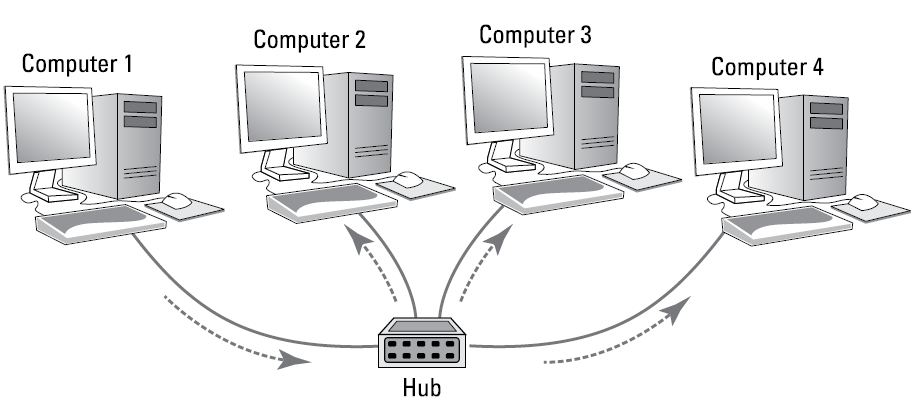
\includegraphics[width=0.7\textwidth]{fig/fig39}
	\caption{Diagram over en repeater og hub forbindelser}
	\label{fig:repeater_hub}
\end{figure}
\noindent En hub er en simpel netværksenhed, der forbinder flere enheder i et LAN (Local Area Network). Den sender data, den modtager, til alle de enheder, der er forbundet til den, uden at tage hensyn til hvilken enhed dataene er beregnet til. Dette medfører ineffektiv dataoverførsel, da unødvendige data sendes til alle tilsluttede enheder. Hubs opererer på det fysiske lag (Layer 1) i OSI-modellen og har begrænset effektivitet sammenlignet med switches, som kun sender data til den specifikke modtager enhed.

\subsection{Switches}
En \textbf{switch} er en mere avanceret netværksenhed, der opererer på lag 2 i OSI-modellen (datalinklaget). I modsætning til hubs, der sender data til alle tilsluttede enheder, sender en switch data kun til den specifikke enhed, som dataene er beregnet til. Dette gøres ved at opretholde en MAC-adressetabel, som kortlægger hver port til en specifik MAC-adresse.
\newline
\newline
\noindent Switches har flere fordele sammenlignet med hubs:
\begin{itemize}
	\item \textbf{Effektivitet:} Fordi switches kun sender data til den specifikke modtager, reduceres unødvendig netværkstrafik, hvilket forbedrer den samlede netværkseffektivitet.
	\item \textbf{Sikkerhed:} Data sendes kun til den tilsigtede modtager, hvilket reducerer risikoen for, at data fanges op af andre enheder på netværket.
	\item \textbf{Ydeevne:} Switches kan håndtere flere samtidige forbindelser uden at forårsage kollisioner, hvilket er et almindeligt problem med hubs.
\end{itemize}
\begin{figure}[!h]
	\centering
	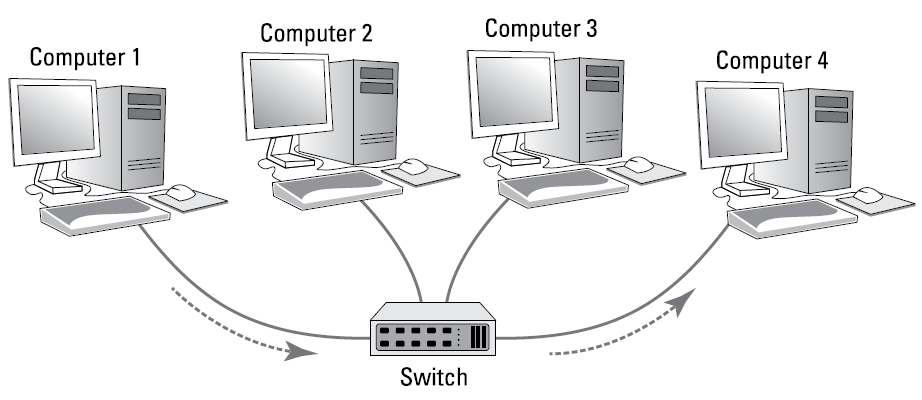
\includegraphics[width=.7\textwidth]{fig/fig40}
	\caption{Switch}
\end{figure}

\subsection{Routere}
En \textbf{router} er en lag 3-enhed, hvilket betyder, at den arbejder på netværkslaget i OSI-modellen. I praksis betyder det, at routere arbejder med IP-adresser. Routere er afgørende for at forbinde forskellige netværk og styre netværkstrafikken mellem dem. En router adskiller sig fra en switch på flere måder:
\begin{itemize}
	\item \textbf{IP-adresser:} Switches arbejder med MAC-adresser og ved ingenting om IP-adresser. I kontrast arbejder routere med IP-adresser.
	\item \textbf{Kommunikation mellem subnetværk:} Routere kan facilitere kommunikation mellem IP-netværk med forskellige subnet. For eksempel, hvis din organisation har et 10.0.100.x netværk og et 192.168.0.x netværk, kan en router muliggøre, at pakker kan rejse fra 10.0.100.x netværket til 192.168.0.x netværket og omvendt.
	\item \textbf{Internetforbindelse:} Routere muliggør også, at et privat netværk kan kommunikere med internettet. For eksempel, hvis du vil forbinde dit netværk til internettet via en bredbåndsudbyder, skal du bruge en router til at udveksle pakker mellem dit private netværk og internettet via den offentlige IP-adresse.
\end{itemize}

\begin{figure}[h!]
	\centering
	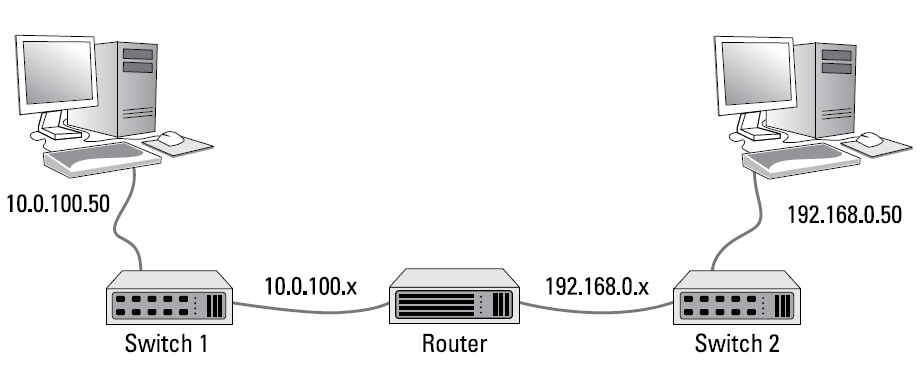
\includegraphics[width=0.8\textwidth]{fig/fig41}
	\caption{To IP-netværk forbundet via en router}
	\label{fig:router}
\end{figure}
\noindent Den grundlæggende funktion af en router er ganske simpel. Overvej det simple netværk afbilledet i figur \ref{fig:router}. Her har en organisation to separate IP-netværk, et med 10.0.100.x subnet og et andet med 192.168.0.x subnet. En router bruges til at forbinde disse to netværk. På begge sider af routeren er der en switch, og hver switch har kun en computer forbundet.
\newline
\newline
\noindent Routeren bruger IP-adresser til at bestemme den bedste vej for data at rejse fra kilden til destinationen. Når en computer på det ene netværk ønsker at sende data til en computer på det andet netværk, sender den først dataene til switchen. Switch 1 videresender dataene til routeren, som derefter bestemmer den bedste vej og sender dataene videre til Switch 2, som til sidst sender dataene til den rigtige destination.

\subsection{Modems}
Et modem (modulator-demodulator) er en enhed, der konverterer digitale data fra en computer til analoge signaler, der kan overføres over telefonlinjer eller kabelnetværk og omvendt. Modemer bruges til at forbinde computere til internettet, især på steder hvor der ikke er tilgængelige bredbåndsforbindelser.

\section{Sammenhæng mellem Netværkshardware}
For at opbygge et effektivt og pålideligt netværk er det vigtigt at forstå, hvordan disse hardwarekomponenter arbejder sammen:
\begin{itemize}
	\item \textbf{Interaktion mellem routere og switches:} Routere forbinder forskellige netværk, mens switches forbinder enheder inden for samme netværk. I et typisk netværk vil en switch forbinde computere og andre enheder i et LAN, og en router vil forbinde dette LAN til internettet.
	\item \textbf{Brug af hubs i små netværk:} Hubs kan anvendes i små netværk med få enheder, hvor effektiviteten ikke er et stort problem. I større netværk vil switches være mere effektive på grund af deres evne til at videresende data specifikt til den tiltænkte modtager.
	\item \textbf{Modemer til internetadgang:} Modemer bruges til at oprette forbindelse til internettet ved at konvertere digitale signaler til analoge og omvendt. De kan arbejde sammen med routere for at distribuere internetadgang til flere enheder i et netværk.
\end{itemize}

\section{Circuit Switching og Packet Switching}
I netværkskommunikation findes der to grundlæggende metoder til dataoverførsel: circuit switching og packet switching. 

\subsection{Circuit Switching}
Circuit switching indebærer oprettelsen af en dedikeret kommunikationskanal mellem to enheder for hele varigheden af en kommunikationssession. Dette er ligesom det traditionelle telefonsystem, hvor en linje er reserveret til en samtale fra start til slut. Fordelen ved circuit switching er, at det sikrer en kontinuerlig og stabil forbindelse, hvilket er ideelt til overførsel af data, der kræver konstant båndbredde. Ulempen er, at denne metode kan være ineffektiv og dyr, da ressourcerne forbliver allokeret, selv når der ikke sendes data.

\subsection{Packet Switching}
Packet switching, derimod, bryder dataene op i mindre pakker, som sendes individuelt gennem netværket. Hver pakke kan tage forskellige ruter til sin destination, afhængigt af netværksforholdene. Ved ankomsten samles pakkerne i den korrekte rækkefølge af modtagerens system. Denne metode er mere effektiv, da netværksressourcerne deles mellem flere brugere, hvilket muliggør optimal udnyttelse af båndbredden. Packet switching anvendes i de fleste moderne datanetværk, såsom internettet, hvor det sikrer fleksibel og pålidelig dataoverførsel.

\subsection{Forbindelsesorienteret og Forbindelsesløs Kommunikation}
Packet-switched netværk kan tilbyde både forbindelsesorienterede og forbindelsesløse kommunikationer. Forbindelsesorienteret kommunikation, som f.eks. TCP (Transmission Control Protocol), etablerer en virtuel forbindelse, hvor dataoverførslerne er struktureret og pålidelige. Forbindelsesløs kommunikation, som f.eks. UDP (User Datagram Protocol), sender data uden at etablere en vedvarende forbindelse, hvilket er hurtigere men mindre pålideligt.

\subsection{Praktisk Anvendelse}
I moderne industrielle netværk anvendes packet switching bredt på grund af dets evne til at håndtere store datamængder effektivt. Denne teknologi gør det muligt at sende data fra mange forskellige kilder samtidigt, hvilket er afgørende for komplekse automationssystemer, hvor forskellige sensorer og enheder konstant kommunikerer.
\newline
\newline
\noindent Sammenfattende er forståelsen af både circuit switching og packet switching vigtig for at kunne designe og implementere effektive netværksløsninger, der opfylder specifikke behov for stabilitet, hastighed og effektivitet.

\section{Media Access Control (MAC) mechanisms}
Medieadgangskontrolmekanismer er essentielle for at regulere, hvordan data sendes og modtages i netværk. Der er tre primære metoder, der anvendes til at styre adgangen til mediet: Master-slave, Token-passing og CSMA/CD.

\subsection{Master-slave (eller forespørgsel-svar) metode}
Master-slave metoden, også kendt som forespørgsel-svar metoden, anvendes ofte i netværk, hvor en central node (master) skal kommunikere med flere underordnede noder (slaver). I denne opsætning styrer masternoden kommunikationen ved at sende forespørgsler til slavenoderne og vente på svar. Processen fungerer således:
\begin{itemize}
	\item Masternoden sender en besked til den første slave i rækken, der enten anmoder om data eller sender data til slaven.
	\item Alle slavenoder modtager beskeden, men kun den node, hvis adresse matcher beskedens destination, reagerer. De andre noder ignorerer beskeden.
	\item Den adresserede slavenode læser beskeden og kontrollerer for eventuelle fejl. Hvis der opdages fejl, såsom uoverensstemmelser i checksummen, afvises beskeden.
	\item Hvis en slave ikke reagerer, forsøger masternoden at kontakte den op til tre gange, før den går videre til den næste slave i rækken.
	\item Denne cyklus fortsætter, indtil alle slavenoder er blevet kontaktet, hvilket udgør en fuld forespørgselscyklus.
\end{itemize}
Fordelen ved denne metode er enkelheden i opsætningen og den fulde kontrol, masternoden har over kommunikationen. Dette gør det nemt at administrere dataflowet, især når hver slave har en forudsigelig mængde data. Ulempen er dog, at systemet kan være ineffektivt, hvis en slave har behov for at sende uforudsete mængder data, eller hvis der opstår behov for hurtig overførsel af kritiske data.

\subsection{Token-passing}
Token-passing er en metode, hvor kontrollen over netværket overføres mellem noder via en særlig besked kaldet en token. Denne metode bruges ofte i netværk, der kræver pålidelig og garanteret dataoverførsel, såsom industrielle kontrolsystemer. Token-passing fungerer på følgende måde:
\begin{itemize}
	\item En node modtager token-beskeden fra en nærliggende node og får dermed kontrol over netværket.
	\item Noden beholder token i en bestemt tidsperiode eller indtil den har sendt sine beskeder.
	\item Noden sender derefter data til andre noder og overfører token til den næste node i rækken.
	\item Denne proces gentages, hvilket sikrer, at alle noder får en chance for at sende data inden for et givet tidsrum.
\end{itemize}
Fordelen ved token-passing er, at det sikrer deterministisk adgang til mediet, hvilket betyder, at alle noder får lige mulighed for at sende data. Dette er især vigtigt i systemer, hvor tidssensitive dataoverførsler er afgørende. Eksempler på netværk, der anvender token-passing, inkluderer Arcnet (stjernetopologi), Modbus (bustopologi) og IBM token ring (ringtopologi).

\subsection{CSMA/CD (Carrier Sense Multiple Access/Collision Detection)}
CSMA/CD er en enkel og effektiv metode til at regulere datatrafik i et netværk. Denne metode anvendes ofte i netværk som Ethernet og fungerer ved, at noder lytter efter ledig båndbredde, før de sender data. CSMA/CD processen er som følger:
\begin{itemize}
	\item En node, der ønsker at sende data, lytter først efter aktivitet på netværket. Hvis netværket er ledigt, begynder noden at sende data.
	\item Under transmissionen sammenligner noden de sendte data med de data, der er til stede på netværket. Hvis der opdages en kollision (dvs. to noder sender samtidig), stopper transmissionen øjeblikkeligt.
	\item De kolliderende noder venter en tilfældig periode, før de forsøger at sende igen, hvilket reducerer risikoen for yderligere kollisioner.
\end{itemize}
CSMA/CD er enkel og effektiv, især i netværk med let trafik. Dog kan metoden blive ineffektiv ved høj trafikbelastning, da kollisioner kan blive hyppige og forsinke dataoverførsler. Det mest almindelige eksempel på CSMA/CD er Ethernet.

\section{Transmissionsteknikker}
Transmissionsteknikker beskriver, hvordan data overføres over et netværk. De to mest anvendte teknikker er baseband og broadband.

\subsection{Baseband}
Baseband transmission er en metode, hvor hele båndbredden af mediet anvendes af en enkelt kommunikationskanal ad gangen. Denne teknik er karakteriseret ved, at signalet sendes direkte uden modulation, hvilket betyder, at den elektriske signalspænding varierer direkte med dataene.
\begin{itemize}
	\item \textbf{Tidssignalering (TDM):} Baseband transmission bruger ofte tidsdeling multiplexing (Time Division Multiplexing, TDM), hvor hver enhed tildeles en bestemt tidslomme til at transmittere data. Dette sikrer, at kun én enhed sender data ad gangen, hvilket eliminerer risikoen for kollisioner.
	\item \textbf{Anvendelse:} Denne metode er almindeligt anvendt i Ethernet-netværk, specielt i det oprindelige 10BASE-T Ethernet, hvor data sendes over twisted pair-kabler uden behov for yderligere modulation.
	\item \textbf{Fordele:}
	\begin{itemize}
		\item Simpel og nem at implementere.
		\item Lav omkostning på grund af enkelheden i udstyr og kabling.
	\end{itemize}
	\item \textbf{Ulemper:}
	\begin{itemize}
		\item Begrænset rækkevidde og båndbredde sammenlignet med broadband.
		\item Ikke velegnet til lange afstande uden brug af repeatere.
	\end{itemize}
\end{itemize}

\subsection{Broadband}
Broadband transmission er en metode, hvor mediets båndbredde opdeles i flere kanaler, som hver især kan transmittere data samtidigt. Dette gøres ved at modulere dataene på forskellige frekvensbærere, hvilket tillader flere signaler at dele samme fysiske medie uden at interferere med hinanden.
\begin{itemize}
	\item \textbf{Frekvensdeling (FDM):} Broadband bruger frekvensdeling multiplexing (Frequency Division Multiplexing, FDM), hvor hver kanal tildeles en specifik frekvensbånd. Dette muliggør parallel transmission af data fra flere enheder.
	\item \textbf{Anvendelse:} Broadband transmission anvendes typisk i kabelnetværk og fiberoptiske netværk, hvor høj båndbredde og lange afstande er nødvendige. Eksempler inkluderer kabel-tv og bredbåndsinternetforbindelser.
	\item \textbf{Fordele:}
	\begin{itemize}
		\item Høj båndbredde, hvilket muliggør hurtigere dataoverførsel.
		\item Kan transmittere over længere afstande uden behov for repeatere.
	\end{itemize}
	\item \textbf{Ulemper:}
	\begin{itemize}
		\item Mere komplekst og dyrere at implementere.
		\item Kræver specialiseret udstyr til modulation og demodulation.
	\end{itemize}
\end{itemize}
Data transmitteres ved at modulere en bærebølge med informationen, hvilket gør det muligt at udnytte større båndbredder og tillade højere dataoverførselshastigheder. Koaksialkabler og optiske fibre er typisk foretrukne medier for FDM på grund af deres høje båndbreddekapacitet.
\newline
\newline
\noindent Disse transmissionsteknikker og medieadgangskontrolmekanismer spiller en afgørende rolle i design og implementering af effektive og pålidelige netværk, både i kommercielle og industrielle applikationer. 
\newline
\newline
\noindent\textbf{Eksempel:} Profinet bruger både Ethernet-standarder (CSMA/CD) og har specifikationer for det fysiske lag, hvilket gør det til en robust løsning for industrielle netværk.

\section{OSI-modellen og dens anvendelse i industrielle netværk}
Open Systems Interconnection (OSI) modellen er en konceptuel ramme, der bruges til at forstå og implementere standarder for netværkskommunikation. Modellen opdeler netværkskommunikation i syv forskellige lag, hvor hvert lag har specifikke funktioner og tjenester. Disse lag er designet til at interagere med hinanden på en standardiseret måde, hvilket muliggør kommunikation mellem forskellige netværksudstyr og protokoller.

\subsection{Lag 1: Fysisk Lag}
Det fysiske lag er det nederste lag i OSI-modellen. Det håndterer den fysiske forbindelse mellem enheder og den faktiske transmission og modtagelse af data i form af elektriske signaler, lys eller radiobølger. Dette lag omfatter hardwarekomponenter som kabler, switches og netværkskort. I industrielle netværk inkluderer dette lag også miljømæssige faktorer som elektromagnetisk interferens og temperaturvariationer, hvilket kan påvirke dataoverførslen.

\subsection{Lag 2: Datalink Lag}
Datalink laget er ansvarligt for pålidelig dataoverførsel mellem to enheder på samme netværk. Det opdeler data i frames og håndterer fejlkorrektion fra det fysiske lag. Datalink laget består af to underlag: Media Access Control (MAC) og Logical Link Control (LLC). I industrielle netværk bruges protokoller som EtherCAT og PROFINET på dette lag for at sikre hurtig og pålidelig dataoverførsel mellem kontroller og feltudstyr.

\subsection{Lag 3: Netværks Lag}
Netværks laget styrer routing af data mellem forskellige netværk. Dette lag opdeler data i pakker og bestemmer den bedste vej til destinationen ved hjælp af routingprotokoller som IP (Internet Protocol). Netværks laget håndterer også logiske adressering. I industrielle netværk bruges ofte avancerede routingteknikker til at sikre, at data når deres destination hurtigt og effektivt, selv i komplekse netværksstrukturer.

\subsection{Lag 4: Transport Lag}
Transport laget er ansvarligt for pålidelig dataoverførsel mellem to endepunkter. Det opdeler data i segmenter og sikrer, at dataene når frem uden fejl og i den rigtige rækkefølge. Protokoller som TCP (Transmission Control Protocol) og UDP (User Datagram Protocol) opererer på dette lag. I industrielle netværk er transportlaget afgørende for at sikre, at kontrolsignaler og dataoverførsler er præcise og pålidelige.

\subsection{Lag 5: Session Lag}
Session laget styrer etablering, vedligeholdelse og afslutning af kommunikationssessioner mellem applikationer. Det sikrer, at sessioner forbliver adskilte og organiserer dataudveksling i sessioner. I industrielle applikationer bruges dette lag til at administrere vedvarende forbindelser mellem kontrolsystemer og deres tilhørende enheder, hvilket sikrer kontinuerlig drift og overvågning.

\subsection{Lag 6: Præsentations Lag}
Præsentations laget er ansvarligt for datatranslation, datakomprimering og datakryptering. Det sørger for, at data, der sendes fra applikationslaget, er i et format, der kan forstås af modtagerens applikationslag. I industrielle netværk kan dette lag være involveret i konvertering af dataformater mellem forskellige systemer og sikring af, at data er korrekt krypteret for sikkerhedsmæssige formål.

\subsection{Lag 7: Applikations Lag}
Applikations laget er det øverste lag i OSI-modellen og fungerer som grænseflade mellem netværkstjenester og applikationssoftware. Det tilbyder tjenester som e-mail, filoverførsel og webbrowseradgang. Protokoller som HTTP, FTP og SMTP opererer på dette lag. I industrielle netværk omfatter dette lag også specialiserede applikationer til processtyring, overvågning og dataindsamling, hvilket gør det muligt for operatører at interagere med og styre industrielle systemer.
\begin{figure}[!h]
	\centering
	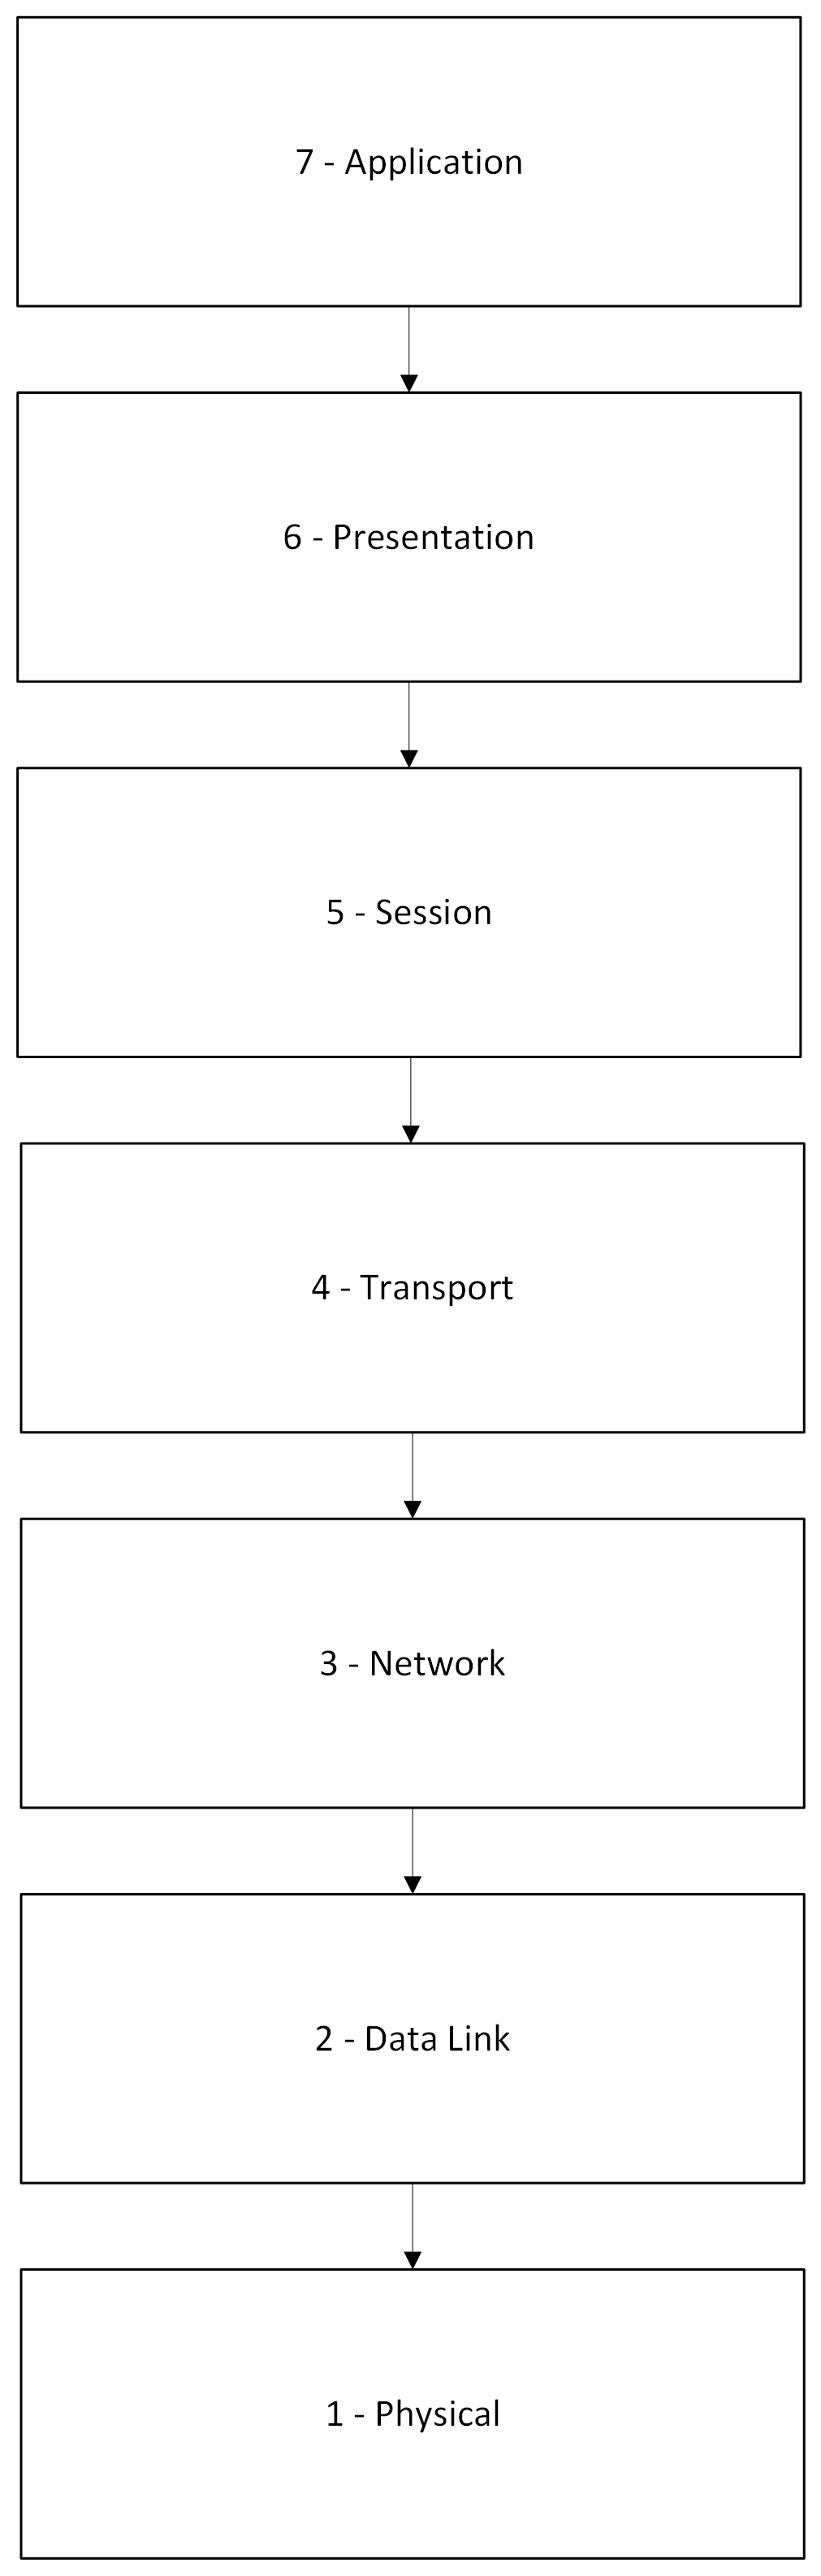
\includegraphics[width=0.3\textwidth]{fig/fig1.png} % Inkluder billedet af OSI-modellen her
	\caption{Illustration af OSI-modellens syv lag}
	\label{fig:osi_model}
\end{figure}

\subsection{Sammenhæng mellem lagene}
Hvert lag i OSI-modellen kommunikerer direkte med de lag, der er umiddelbart over og under det. Data, der sendes fra en applikation, bevæger sig ned gennem lagene, hvor hver lag tilføjer sine egne specifikke oplysninger (f.eks. headers og trailers), inden de transmitteres over netværket. Ved modtagelse bevæger dataene sig op gennem lagene, hvor hver lag fjerner sine tilsvarende oplysninger og videresender de relevante data til det næste lag.
\begin{itemize}
	\item \textbf{Fordele ved OSI-modellen:}
	\begin{itemize}
		\item Standardisering: Tilbyder en standardiseret ramme for netværkskommunikation.
		\item Interoperabilitet: Muliggør interoperabilitet mellem forskellige netværksprodukter og -teknologier.
		\item Modularitet: Tillader udvikling og fejlfinding af individuelle lag uden at påvirke de andre lag.
	\end{itemize}
\end{itemize}
For en visuel forståelse, se Figur \ref{fig:osi_model}, som illustrerer OSI-modellens syv lag og deres funktioner.

\subsection{Anvendelse af OSI-modellen i industrielle netværk}
I industrielle netværk anvendes OSI-modellen til at designe og implementere netværksinfrastrukturer, der opfylder specifikke krav til pålidelighed, sikkerhed og effektivitet. Hvert lag i OSI-modellen bidrager til den samlede funktionalitet og ydeevne af netværket.
\newline
\newline
\noindent\textbf{Eksempel på Anvendelse: PROFINET}
PROFINET er en industriel Ethernet-standard, der bruger OSI-modellen som grundlag. PROFINET opererer primært på datalinklaget (Lag 2) og netværkslaget (Lag 3), hvor det leverer realtidskommunikation og understøtter komplekse industrielle applikationer.
\newline
\newline
\noindent\textbf{Fordele ved at Bruge OSI-modellen}
Anvendelse af OSI-modellen i industrielle netværk har flere fordele:
\begin{itemize}
	\item \textbf{Standardisering:} OSI-modellen fremmer brugen af standardprotokoller, hvilket gør det lettere at integrere forskellige enheder og systemer fra forskellige producenter.
	\item \textbf{Fejlfinding:} Ved at opdele netværksfunktioner i adskilte lag bliver det lettere at identificere og isolere problemer.
	\item \textbf{Fleksibilitet:} OSI-modellen tillader udskiftning og opgradering af individuelle lag uden at påvirke hele netværket.
	\item \textbf{Pålidelighed:} Ved at implementere specifikke funktioner på hvert lag kan netværket opnå højere pålidelighed og ydeevne.
\end{itemize}
\textbf{Implementeringsstrategier}
Ved implementering af industrielle netværk skal ingeniører og teknikere:
\begin{itemize}
	\item Vælge passende protokoller og teknologier for hvert lag baseret på specifikke behov.
	\item Sikre, at alle lag i OSI-modellen er korrekt konfigureret og integreret.
	\item Udføre grundig testning og validering for at sikre, at netværket fungerer som forventet.
\end{itemize}
\noindent OSI-modellen er et uvurderligt værktøj i planlægning, design og implementering af industrielle netværk. Ved at forstå og anvende denne model kan netværksingeniører skabe robuste, sikre og effektive netværk, der opfylder moderne industrikrav.

\section{TCP/IP-modellen}
TCP/IP-modellen (Transmission Control Protocol/Internet Protocol) er en konceptuel model og et sæt af kommunikationsprotokoller, der bruges til at forbinde enheder på internettet. Modellen opdeler netværkskommunikation i fire forskellige lag, som tilsammen muliggør dataudveksling mellem netværk.

\paragraph{Lag 1: Netværksadgangslaget}
Dette lag omfatter de protokoller og teknologier, der anvendes til fysisk at forbinde og overføre data mellem enheder på samme netværk. Det svarer til OSI-modellens fysiske og datalink-lag. Protokoller og teknologier i dette lag inkluderer Ethernet, Wi-Fi, og ARP (Address Resolution Protocol).

\paragraph{Lag 2: Internetlaget}
Internetlaget er ansvarligt for routing af data mellem forskellige netværk. Dette lag tilsvarer OSI-modellens netværkslag og bruger IP (Internet Protocol) til at bestemme, hvordan pakker skal dirigeres fra afsender til modtager. Andre vigtige protokoller i dette lag inkluderer ICMP (Internet Control Message Protocol) og IGMP (Internet Group Management Protocol).

\paragraph{Lag 3: Transportlaget}
Transportlaget sørger for pålidelig dataoverførsel mellem to endepunkter. Dette lag svarer til OSI-modellens transportlag og omfatter to primære protokoller: TCP (Transmission Control Protocol) og UDP (User Datagram Protocol). TCP er ansvarlig for at sikre, at data leveres uden fejl og i den rigtige rækkefølge, mens UDP giver en hurtigere, men mindre pålidelig overførsel.

\paragraph{Lag 4: Applikationslaget}
Applikationslaget er det øverste lag i TCP/IP-modellen og omfatter alle de protokoller, der anvendes af applikationer til at kommunikere over netværket. Dette lag tilsvarer de tre øverste lag i OSI-modellen (session, præsentation, og applikation). Eksempler på protokoller i dette lag inkluderer HTTP (HyperText Transfer Protocol), FTP (File Transfer Protocol), SMTP (Simple Mail Transfer Protocol), og DNS (Domain Name System).

\paragraph{Sammenligning med OSI-modellen}
TCP/IP-modellen og OSI-modellen er begge designet til at hjælpe med forståelsen af netværkskommunikation. Mens OSI-modellen har syv lag, har TCP/IP-modellen kun fire. OSI-modellen bruges ofte som en teoretisk ramme, mens TCP/IP-modellen er praktisk og implementeret i de fleste netværk i dag.

\paragraph{Fordele ved TCP/IP-modellen}
Robusthed: TCP/IP er designet til at være robust og pålidelig, selv i tilfælde af fejl og tab af data.
Skalerbarhed: Modellen er meget skalerbar og kan håndtere et stort antal enheder og netværk.
Interoperabilitet: TCP/IP tillader kommunikation mellem enheder fra forskellige producenter og operativsystemer.
Standardisering: TCP/IP er en de facto standard for netværkskommunikation, hvilket gør det universelt accepteret og brugt.

\paragraph{Anvendelser af TCP/IP-modellen}
TCP/IP-modellen anvendes bredt i moderne netværk, herunder internettet, lokale netværk (LAN), og virksomhedsintranets. Den understøtter et bredt udvalg af applikationer, fra web browsing og e-mail til filoverførsel og streamingtjenester.

\section{Forskellen mellem OSI- og TCP/IP-modellen}
\section*{Introduktion}
I netværkskommunikation er OSI- og TCP/IP-modellerne to fundamentale rammer, der hjælper med at forstå, hvordan data overføres mellem enheder. OSI-modellen er en konceptuel model, der primært bruges til undervisning og standardisering, mens TCP/IP-modellen er den praktisk anvendte model på internettet i dag.

\section{OSI-modellen}
\subsection{Struktur}
OSI-modellen (Open Systems Interconnection) består af syv lag, der hver især har specifikke funktioner:
\begin{enumerate}
	\item \textbf{Fysisk Lag:} Transmission af rå bitstrømme over et fysisk medium.
	\item \textbf{Datalink Lag:} Sikrer pålidelig dataoverførsel over et fysisk link.
	\item \textbf{Netværks Lag:} Routing af data mellem forskellige netværk.
	\item \textbf{Transport Lag:} Sikrer pålidelig dataoverførsel mellem to endepunkter.
	\item \textbf{Session Lag:} Styrer etablering, vedligeholdelse og afslutning af kommunikationssessioner.
	\item \textbf{Præsentations Lag:} Datatranslation, datakomprimering og datakryptering.
	\item \textbf{Applikations Lag:} Grænseflade mellem netværkstjenester og applikationssoftware.
\end{enumerate}

\subsection{Formål og Anvendelse}
OSI-modellen blev udviklet af ISO (International Organization for Standardization) som en teoretisk ramme for standardisering af netværkskommunikation. Den bruges hovedsageligt i uddannelsesmiljøer til at forstå og designe netværksprotokoller og -systemer.

\section{TCP/IP-modellen}
\subsection{Struktur}
TCP/IP-modellen (Transmission Control Protocol/Internet Protocol) har fire lag, der er designet til praktisk brug i netværkskommunikation:
\begin{enumerate}
	\item \textbf{Netværksadgangslaget:} Håndterer fysisk forbindelse og datalink, herunder hardwarekomponenter som kabler og switches.
	\item \textbf{Internetlaget:} Ansvarlig for routing af data mellem forskellige netværk ved hjælp af IP (Internet Protocol).
	\item \textbf{Transportlaget:} Pålidelig dataoverførsel mellem to endepunkter med protokoller som TCP og UDP.
	\item \textbf{Applikationslaget:} Protokoller, der anvendes af applikationer til netværkskommunikation, som HTTP, FTP, SMTP.
\end{enumerate}

\subsection{Formål og Anvendelse}
TCP/IP-modellen blev udviklet af det amerikanske forsvarsministerium (DoD) for at understøtte netværkskommunikation i ARPANET, som var forløberen til internettet. Denne model er praktisk anvendt og designet til at lette kommunikation over forskellige typer netværk, og den er grundlaget for moderne internetinfrastruktur.

\section{Sammenligning mellem OSI og TCP/IP}
\subsection{Lagstruktur}
\begin{itemize}
	\item \textbf{OSI-modellen:} Består af syv detaljerede lag, der opdeler netværkskommunikation i specifikke funktioner.
	\item \textbf{TCP/IP-modellen:} Har fire lag, hvor flere funktioner fra OSI-modellen kombineres. For eksempel dækker Netværksadgangslaget i TCP/IP både det fysiske lag og datalinklaget i OSI-modellen.
\end{itemize}

\subsection{Abstraktionsniveau og Brug}
\begin{itemize}
	\item \textbf{OSI-modellen:} Tilbyder en detaljeret og lagdelt tilgang, der primært anvendes som en teoretisk reference for netværkskommunikation.
	\item \textbf{TCP/IP-modellen:} Er mere praktisk og bruges i reel netværkskommunikation og internetprotokoller.
\end{itemize}

\subsection{Udvikling og Anvendelse}
\begin{itemize}
	\item \textbf{OSI-modellen:} Udviklet af en international standardiseringsorganisation og anvendes mest til pædagogiske formål.
	\item \textbf{TCP/IP-modellen:} Udviklet af det amerikanske forsvar og er den mest anvendte model i moderne netværkskommunikation, især på internettet.
\end{itemize}

\section{Opsummering: OSI vs TCP/IP}
OSI-modellen giver en teoretisk og detaljeret ramme, der er nyttig for undervisning og standardisering, mens TCP/IP-modellen er praktisk anvendt i moderne netværksinfrastruktur, især på internettet. Sammen supplerer disse modeller hinanden og giver en omfattende forståelse af netværkskommunikation.

\chapter{ Ethernet-teknologier og Protokoller}
\section{Internet Protocol version 4 (IPv4)}
Internetprotokollen (IP) er kernen i TCP/IP-protokolsuiten. IP er primært ansvarlig for routing af pakker mod deres destination, fra router til router. Denne routing udføres på basis af IP-adresser, som er indlejret i headeren, der er knyttet til hver pakke, der videresendes af IP.
\newline\newline\noindent 
Den mest udbredte version af IP i dag er version 4 (IPv4), som bruger en 32-bit adresse. En IPv4-adresse består af fire oktetter (8-bit segmenter), adskilt af punktummer. For eksempel er \texttt{192.168.1.1} en gyldig IPv4-adresse.
\newline\newline\noindent 
IPv4 er ved at nå slutningen af sin levetid, hovedsageligt på grund af det begrænsede antal tilgængelige adresser. For at imødegå dette problem er version 6 (IPv6 eller IPng) blevet udviklet, som bruger en 128-bit adresse. Selvom denne vejledning primært fokuserer på IPv4 for at forklare de grundlæggende processer, vil den også give en introduktion til IPv6.

\subsection{Kilde til IP-adresser}
En IP-adresse er en unik numerisk identifikator, der tildeles hver enhed, der er forbundet til et computernetværk, der bruger internetprotokollen til kommunikation. Disse adresser stammer fra Internet Assigned Numbers Authority (IANA), som er ansvarlig for at fordele dem globalt. IANA har delegeret denne opgave til tre regionale internetregistre (RIRs):
\begin{itemize}
	\item \textbf{APNIC:} Asien og Stillehavsområdet (\url{http://www.apnic.net})
	\item \textbf{ARIN:} Nordamerika og dele af Caribien (\url{http://www.arin.net})
	\item \textbf{RIPE NCC:} Europa, Mellemøsten og dele af Centralasien (\url{http://www.ripe.net})
\end{itemize}
RIR'erne tildeler blokke af IP-adresser til internetudbydere (ISPs), som derefter tildeler dem til deres kunder. For at kunne oprette forbindelse til internettet skal en enhed have en gyldig IP-adresse. Enheder, der ikke er forbundet til internettet, kan bruge private IP-adresser. Disse adresser er ikke unikke globalt og kan derfor ikke bruges til at kommunikere direkte med enheder på internettet.

\subsection{IP-adressens rolle i netværkskommunikation}
En IP-adresse fungerer som en digital postadresse for enheder, der er forbundet til et netværk. Den gør det muligt at identificere hver enkelt enhed og dirigere data mellem dem pålideligt. Uden IP-adresser ville internettet og andre netværk ikke kunne fungere.

\paragraph{IP-adressens hovedfunktioner}
\begin{itemize}
	\item \textbf{Unik identifikation:} Hver enhed på et netværk får tildelt en unik IP-adresse, der adskiller den fra alle andre enheder. Det er lidt ligesom et CPR-nummer for mennesker.
	\item \textbf{Routing af data:} Når du sender data over et netværk, f.eks. en e-mail eller besøger en hjemmeside, bruges IP-adressen til at bestemme den bedste rute for dataene at følge fra din enhed til destinationen.
	\item \textbf{Internetkommunikation:} For at din computer, smartphone eller anden enhed kan kommunikere med andre enheder på internettet, skal den have en gyldig og unik IP-adresse.
\end{itemize}

\subsection{IP-adresser vs. MAC-adresser}
Du har måske hørt om MAC-adresser (også kaldet hardware-adresser). De er også unikke identifikatorer for netværksenheder, men de er mere som et serienummer, der er indbygget i enheden fra fabrikken. MAC-adresser bruges primært til kommunikation inden for et lokalt netværk (LAN), hvor alle enheder er direkte forbundet.
\newline
\newline
\noindent IP-adresser er derimod nødvendige for kommunikation på tværs af forskellige netværk, som f.eks. internettet. De er mere fleksible end MAC-adresser, da de kan ændres, hvis enhed flyttes til et andet netværk eller skifter internetudbyder.

\paragraph{Hvordan IP-adresser og MAC-adresser arbejder sammen}
Når du sender data til en anden enhed på internettet, sker der en oversættelse mellem IP-adressen og MAC-adressen. Din enhed bruger IP-adressen til at finde den rigtige destination på internettet. Når dataene når det lokale netværk, hvor destinationen befinder sig, bruges MAC-adressen til at levere dataene til den specifikke enhed.
\newline\newline\noindent 
Denne oversættelse mellem IP- og MAC-adresser sker automatisk ved hjælp af en protokol kaldet ARP (Address Resolution Protocol).

\subsection{Netværks-ID og Host-ID}
En IPv4-adresse kan opdeles i to dele: Netværks-ID og Host-ID. Netværks-ID identificerer det overordnede netværk, mens Host-ID identificerer en specifik enhed inden for det netværk. Subnetmasken bruges til at bestemme, hvilken del af adressen der er netværks-ID, og hvilken der er Host-ID.
\newline\newline\noindent 
\textbf{Eksempel:}
\newline\noindent For IP-adressen \texttt{192.168.1.10} med subnetmasken \texttt{255.255.255.0}:
\begin{itemize}
	\item Netværks-ID: \texttt{192.168.1.0}
	\item Host-ID: \texttt{10}
\end{itemize}

\subsection{Adresseklasser}
IPv4-adresser er opdelt i fem klasser (A, B, C, D, og E) baseret på de første bits af adressen:

\begin{itemize}
	\item \textbf{Klasse A:} 0.0.0.0 til 127.255.255.255 (stor mængde hosts pr. netværk)
	\item \textbf{Klasse B:} 128.0.0.0 til 191.255.255.255 (medium mængde hosts pr. netværk)
	\item \textbf{Klasse C:} 192.0.0.0 til 223.255.255.255 (lille mængde hosts pr. netværk)
	\item \textbf{Klasse D:} 224.0.0.0 til 239.255.255.255 (multicast-adresser)
	\item \textbf{Klasse E:} 240.0.0.0 til 255.255.255.255 (eksperimentelle adresser)
\end{itemize}

\subsection{Bestemmelse af adresseklasse ved inspektion}
Adresseklassen kan bestemmes ved at inspicere de første bits i en IPv4-adresse:
\begin{itemize}
	\item Klasse A: Første bit er 0 (f.eks. \texttt{1.0.0.0} til \texttt{127.255.255.255})
	\item Klasse B: Første to bits er 10 (f.eks. \texttt{128.0.0.0} til \texttt{191.255.255.255})
	\item Klasse C: Første tre bits er 110 (f.eks. \texttt{192.0.0.0} til \texttt{223.255.255.255})
	\item Klasse D: Første fire bits er 1110 (f.eks. \texttt{224.0.0.0} til \texttt{239.255.255.255})
	\item Klasse E: Første fire bits er 1111 (f.eks. \texttt{240.0.0.0} til \texttt{255.255.255.255})
\end{itemize}

\subsection{Antal netværk og værter pr. adresseklasse}
Antallet af netværk og værter i hver adresseklasse varierer:

\begin{itemize}
	\item \textbf{Klasse A:} 128 netværk, 16.777.214 værter pr. netværk
	\item \textbf{Klasse B:} 16.384 netværk, 65.534 værter pr. netværk
	\item \textbf{Klasse C:} 2.097.152 netværk, 254 værter pr. netværk
\end{itemize}

\section{Subnetmasker}
En subnetmaske er en 32-bit adresse, der opdeler en IP-adresse i netværks- og hostdele. Eksempler:

\begin{itemize}
	\item \texttt{255.255.255.0} (CIDR notation: /24) - 24 bits til netværksdelen og 8 bits til hostdelen.
	\item \texttt{255.255.0.0} (CIDR notation: /16) - 16 bits til netværksdelen og 16 bits til hostdelen.
\end{itemize}

\noindent \textbf{Eksempel:}
\newline\noindent For IP-adressen \texttt{192.168.1.10} med subnetmasken \texttt{255.255.255.0}:
\begin{itemize}
	\item Netværks-ID: \texttt{192.168.1.0}
	\item Host-ID: \texttt{10}
\end{itemize}

\subsection{Subnetting}
Subnetting er processen med at opdele et større netværk i mindre subnets for at forbedre effektiviteten og sikkerheden. Subnetting bruger subnetmasker til at opdele IP-adressen i mindre, håndterbare segmenter.

\subsection{Hvorfor subnetting?}
Subnetting bruges til at:
\begin{itemize}
	\item Reducere netværkstrafik ved at mindske antallet af broadcasts.
	\item Forbedre sikkerheden ved at isolere segmenter af netværket.
	\item Effektivisere IP-adressebrug ved at opdele store netværk i mindre, lettere håndterbare subnets.
\end{itemize}

\subsection{Matematisk proces for subnetting}
For at opdele et netværk i subnets, følg disse trin:
\begin{enumerate}
	\item Bestem antallet af nødvendige subnets eller hosts pr. subnet.
	\item Beregn subnetmasken:
	\begin{itemize}
		\item Antallet af bits, der skal lånes fra host-delen, bestemmes af antallet af nødvendige subnets.
		\item Brug formelen \(2^n \geq antal\) \textit{subnets}, hvor \(n\) er antallet af lånte bits.
		\item Subnetmasken kan derefter beregnes ved at tilføje de lånte bits til netværks-delen af den oprindelige subnetmaske.
	\end{itemize}
	\item Beregn antallet af hosts pr. subnet:
	\begin{itemize}
		\item Brug formelen \(2^h - 2\), hvor \(h\) er antallet af bits i host-delen.
	\end{itemize}
	\item Identificer subnet-ID'er:
	\begin{itemize}
		\item Subnet-ID'er kan identificeres ved at øge subnet-bitsene trinvis.
	\end{itemize}
\end{enumerate}

\subsubsection{Eksempel 1: Subnetting et Class C-netværk}
\textbf{Scenarie:} En virksomhed har et Class C-netværk \texttt{192.168.1.0/24} og ønsker at opdele dette netværk i 4 mindre subnets for at adskille forskellige afdelinger.

\textbf{Beregninger:}
\begin{enumerate}
	\item Bestem antallet af nødvendige subnets: Virksomheden ønsker 4 subnets.
	\item Beregn subnetmasken:
	\begin{itemize}
		\item Antallet af nødvendige bits for subnetting kan beregnes med \(2^n \geq 4\), hvor \(n\) er antallet af lånte bits. Så \(n = 2\).
		\item Den oprindelige subnetmaske er \texttt{255.255.255.0} (/24). Ved at låne 2 bits fra host-delen, bliver den nye subnetmaske \texttt{255.255.255.192} (/26).
	\end{itemize}
	\item Beregn antallet af hosts pr. subnet:
	\begin{itemize}
		\item Antallet af hosts pr. subnet kan beregnes med \(2^h - 2\), hvor \(h\) er antallet af bits i host-delen. For /26 subnetmasken har vi 6 bits til hosts, så \(2^6 - 2 = 62\) hosts pr. subnet.
	\end{itemize}
	\item Identificer subnet-ID'er:
	\begin{itemize}
		\item Første subnet: \texttt{192.168.1.0/26} (hosts: \texttt{192.168.1.1} til \texttt{192.168.1.62})
		\item Andet subnet: \texttt{192.168.1.64/26} (hosts: \texttt{192.168.1.65} til \texttt{192.168.1.126})
		\item Tredje subnet: \texttt{192.168.1.128/26} (hosts: \texttt{192.168.1.129} til \texttt{192.168.1.190})
		\item Fjerde subnet: \texttt{192.168.1.192/26} (hosts: \texttt{192.168.1.193} til \texttt{192.168.1.254})
	\end{itemize}
\end{enumerate}

\subsubsection{Eksempel 2: Subnetting et Class B-netværk}
\textbf{Scenarie:} En skole har et Class B-netværk \texttt{172.16.0.0/16} og ønsker at opdele dette netværk i 16 subnets for at adskille forskellige bygninger.

\textbf{Beregninger:}
\begin{enumerate}
	\item Bestem antallet af nødvendige subnets: Skolen ønsker 16 subnets.
	\item Beregn subnetmasken:
	\begin{itemize}
		\item Antallet af nødvendige bits for subnetting kan beregnes med \(2^n \geq 16\), hvor \(n\) er antallet af lånte bits. Så \(n = 4\).
		\item Den oprindelige subnetmaske er \texttt{255.255.0.0} (/16). Ved at låne 4 bits fra host-delen, bliver den nye subnetmaske \texttt{255.255.240.0} (/20).
	\end{itemize}
	\item Beregn antallet af hosts pr. subnet:
	\begin{itemize}
		\item Antallet af hosts pr. subnet kan beregnes med \(2^h - 2\), hvor \(h\) er antallet af bits i host-delen. For /20 subnetmasken har vi 12 bits til hosts, så \(2^{12} - 2 = 4094\) hosts pr. subnet.
	\end{itemize}
	\item Identificer subnet-ID'er:
	\begin{itemize}
		\item Første subnet: \texttt{172.16.0.0/20} (hosts: \texttt{172.16.0.1} til \texttt{172.16.15.254})
		\item Andet subnet: \texttt{172.16.16.0/20} (hosts: \texttt{172.16.16.1} til \texttt{172.16.31.254})
		\item Tredje subnet: \texttt{172.16.32.0/20} (hosts: \texttt{172.16.32.1} til \texttt{172.16.47.254})
		\item Fortsæt for de resterende subnets: \texttt{172.16.48.0/20}, \texttt{172.16.64.0/20}, osv.
	\end{itemize}
\end{enumerate}

\subsubsection{Eksempel 3: Subnetting et Class A-netværk}
\textbf{Scenarie:} En stor virksomhed har et Class A-netværk \texttt{10.0.0.0/8} og ønsker at opdele dette netværk i 256 subnets for at adskille forskellige afdelinger og lokationer.
\newline\newline\noindent
\textbf{Beregninger:}
\begin{enumerate}
	\item Bestem antallet af nødvendige subnets: Virksomheden ønsker 256 subnets.
	\item Beregn subnetmasken:
	\begin{itemize}
		\item Antallet af nødvendige bits for subnetting kan beregnes med \(2^n \geq 256\), hvor \(n\) er antallet af lånte bits. Så \(n = 8\).
		\item Den oprindelige subnetmaske er \texttt{255.0.0.0} (/8). Ved at låne 8 bits fra host-delen, bliver den nye subnetmaske \texttt{255.255.0.0} (/16).
	\end{itemize}
	\item Beregn antallet af hosts pr. subnet:
	\begin{itemize}
		\item Antallet af hosts pr. subnet kan beregnes med \(2^h - 2\), hvor \(h\) er antallet af bits i host-delen. For /16 subnetmasken har vi 16 bits til hosts, så \(2^{16} - 2 = 65534\) hosts pr. subnet.
	\end{itemize}
	\item Identificer subnet-ID'er:
	\begin{itemize}
		\item Første subnet: \texttt{10.0.0.0/16} (hosts: \texttt{10.0.0.1} til \texttt{10.0.255.254})
		\item Andet subnet: \texttt{10.0.1.0/16} (hosts: \texttt{10.0.1.1} til \texttt{10.0.1.254})
		\item Tredje subnet: \texttt{10.0.2.0/16} (hosts: \texttt{10.0.2.1} til \texttt{10.0.2.254})
		\item Fortsæt for de resterende subnets: \texttt{10.0.3.0/16}, \texttt{10.0.4.0/16}, osv.
	\end{itemize}
\end{enumerate}

\subsubsection{Eksempel 4: Subnetting et Class B-netværk til små undernet}
\textbf{Scenarie:} En IT-afdeling har et Class B-netværk \texttt{172.16.0.0/16} og ønsker at opdele dette netværk i mindre subnets, hver med plads til 30 hosts.
\newline\newline\noindent
\textbf{Beregninger:}
\begin{enumerate}
	\item Bestem antallet af nødvendige subnets: For at have subnets med 30 hosts skal vi bruge en subnetmaske, der giver mindst 30 hosts pr. subnet.
	\item Beregn subnetmasken:
	\begin{itemize}
		\item Antallet af nødvendige bits for hosts kan beregnes med \(2^h - 2 \geq 30\), hvor \(h\) er antallet af bits i host-delen. Så \(h = 5\).
		\item Den oprindelige subnetmaske er \texttt{255.255.0.0} (/16). Ved at låne 11 bits fra host-delen (fordi vi har 16 bits til hosts i et Class B-netværk, og vi skal efterlade 5 bits til hosts), bliver den nye subnetmaske \texttt{255.255.255.224} (/27).
	\end{itemize}
	\item Beregn antallet af subnets:
	\begin{itemize}
		\item Antallet af subnets kan beregnes med \(2^n\), hvor \(n\) er antallet af lånte bits. For /27 subnetmasken har vi lånt 11 bits, så \(2^{11} = 2048\) subnets.
	\end{itemize}
	\item Identificer subnet-ID'er:
	\begin{itemize}
		\item Første subnet: \texttt{172.16.0.0/27} (hosts: \texttt{172.16.0.1} til \texttt{172.16.0.30})
		\item Andet subnet: \texttt{172.16.0.32/27} (hosts: \texttt{172.16.0.33} til \texttt{172.16.0.62})
		\item Tredje subnet: \texttt{172.16.0.64/27} (hosts: \texttt{172.16.0.65} til \texttt{172.16.0.94})
		\item Fortsæt for de resterende subnets: \texttt{172.16.0.96/27}, \texttt{172.16.0.128/27}, osv.
	\end{itemize}
\end{enumerate}

\section{IP-adressering: Klassebaseret og Private vs Internet-unikke Adresser}
IP-adressering er grundlaget for at identificere enheder i et netværk, både lokalt og globalt. Historisk set blev IP-adresser opdelt i faste klasser (A, B, C) baseret på de første bits i adressen. Dette system blev kaldt klassebaseret adressering.

\subsection{Klassebaseret Adressering}
Klassebaseret adressering inddeler IP-adresser i følgende klasser:

\begin{itemize}
	\item \textbf{Klasse A:} Bruges til netværk med et meget stort antal værter. Adresserne spænder fra 1.0.0.0 til 126.0.0.0.
	\item \textbf{Klasse B:} Bruges til netværk med et mellemstort antal værter. Adresserne spænder fra 128.0.0.0 til 191.255.0.0.
	\item \textbf{Klasse C:} Bruges til netværk med et mindre antal værter. Adresserne spænder fra 192.0.0.0 til 223.255.255.0.
\end{itemize}
Dette system er nu stort set erstattet af klasseløs adressering (CIDR), som giver en mere fleksibel og effektiv udnyttelse af adressepladsen.

\subsection{Private vs Internet-unikke IP-adresser}
Inden for det klassebaserede system blev bestemte adresser reserveret som private IP-adresser, som kun bruges inden for lokale netværk og ikke er routable på internettet. Disse adresser er defineret i RFC 1918 og falder ind under følgende områder:
\begin{itemize}
	\item \textbf{Klasse A:} 10.0.0.0 til 10.255.255.255
	\item \textbf{Klasse B:} 172.16.0.0 til 172.31.255.255
	\item \textbf{Klasse C:} 192.168.0.0 til 192.168.255.255
\end{itemize}
\noindent Private IP-adresser bruges typisk i lokale netværk, som f.eks. i hjem eller små kontorer, hvor enheder som computere og printere kommunikerer internt. En hjemme-router kan f.eks. bruge en privat IP-adresse som \texttt{192.168.1.1} for at give netværksadgang til enheder på det lokale netværk.
\newline\newline\noindent
Offentlige eller internet-unikke IP-adresser, derimod, er routable på internettet og bruges til at identificere enheder globalt. Disse adresser er nødvendige for at kommunikere med enheder uden for det lokale netværk.

\section{Classless Inter-Domain Routing (CIDR)}

\subsection{Redegørelse}
CIDR blev introduceret i 1993 som en metode til at forbedre effektiviteten og fleksibiliteten af IP-adressetildelingen. I modsætning til den klassebaserede IP-adressetildeling, som begrænsede antallet af mulige netværk og undernet, tillader CIDR en mere nuanceret og effektiv fordeling af IP-adresser. CIDR bruger en teknik kendt som "subnetting", hvor en enkelt IP-adresse kan opdeles i flere mindre netværkssegmenter ved hjælp af en variabel subnetmaske. Dette reducerer spildet af IP-adresser og giver netværksadministratorer mulighed for at tilpasse størrelsen af netværk og undernet til specifikke behov.

\subsection{Anvendelse}
I praksis anvendes CIDR til at skabe mindre og mere håndterbare netværk, hvilket forbedrer netværkseffektiviteten og -sikkerheden. Det gør det muligt for netværksadministratorer at opdele et stort netværk i flere undernet, hvilket kan hjælpe med at organisere netværkstrafik og begrænse omfanget af netværksforstyrrelser. CIDR er også afgørende for routing, da det reducerer størrelsen af routingtabeller i internettets backbone-routere, hvilket gør internettet mere skalerbart og effektivt.

\subsection{Eksempel}
En adresse som \texttt{192.168.0.0/23} dækker adresserne \\\texttt{192.168.0.0} til \texttt{192.168.1.255}, hvilket giver 512 adresser. Ved at bruge CIDR kan netværksadministratorer tilpasse subnetmasken efter behovene for specifikke netværkssegmenter.

\subsection{Analyse}
Effektiviteten af CIDR kan ses i dets evne til at forlænge levetiden af IPv4-adresserummet. Uden CIDR ville IPv4-adresserummet være blevet udtømt meget hurtigere. Denne metode har også haft en afgørende betydning for udviklingen af internettet, da det har gjort det muligt at håndtere en eksponentiel stigning i antallet af netværksenheder. Dog introducerer CIDR kompleksitet i netværksdesign og -forvaltning, hvilket kræver en mere dybtgående forståelse af IP-netværk og subnetting.

\subsection{Perspektivering}
Med overgangen til IPv6, hvor der er et langt større antal tilgængelige adresser, forbliver principperne bag CIDR relevante. IPv6-adressering indebærer en lignende logik for subnetting og effektiv adresseallokering, selvom den implementerer det på en anden måde på grund af IPv6-adressernes størrelse. Derudover understreger CIDR's succes nødvendigheden af kontinuerlig innovation i netværksteknologier for at imødekomme de stadigt skiftende krav til internettet og digital kommunikation.

\section{IPv4 Header-struktur}
\begin{table}[h]
	\centering
	\begin{tabular}{|c|c|c|c|}
		\hline
		\multicolumn{4}{|c|}{\textbf{IPv4 Header}} \\ \hline
		\textbf{Ver} & \textbf{IHL} & \textbf{Type of Service} & \textbf{Total Length} \\ \hline
		\multicolumn{2}{|c|}{\textbf{Identification}} & \textbf{Flags} & \textbf{Fragment Offset} \\ \hline
		\textbf{Time to Live} & \textbf{Protocol} & \multicolumn{2}{c|}{\textbf{Header Checksum}} \\ \hline
		\multicolumn{4}{|c|}{\textbf{Source Address}} \\ \hline
		\multicolumn{4}{|c|}{\textbf{Destination Address}} \\ \hline
		\multicolumn{4}{|c|}{\textbf{Options + Padding (if any)}} \\ \hline
	\end{tabular}
	\caption{IPv4 Header-struktur}
	\label{tab:ipv4-header}
\end{table}

\noindent IPv4-headeren indeholder vigtige oplysninger for routing og levering af pakker. Den består af flere felter, herunder:

\begin{itemize}
	\item \textbf{Version (Ver):} 4 bits, som angiver versionen af IP-protokollen. I dette tilfælde er det version 4.
	\item \textbf{Header længde (IHL):} 4 bits, som angiver længden af IP-headeren i 32-bit ord. Minimum værdien er 5, hvilket repræsenterer 20 bytes.
	\item \textbf{Type af service (ToS):} 8 bits, som indikerer parametrene for den ønskede servicekvalitet, såsom forsinkelse, gennemstrømning og pålidelighed.
	\item \textbf{Total længde:} 16 bits, som angiver den totale længde af datagrammet, inklusive header og data. Maksimum længden er 65.535 bytes.
	\item \textbf{Identifikation:} 16 bits, som identificerer hvert datagram unikt. Det er nyttigt ved fragmentering for at identificere og genopbygge datagrammer.
	\item \textbf{Flags og fragment offset:} 16 bits, som indeholder 3 flags og 13-bit fragment offset. Flags inkluderer DF (Don’t Fragment) og MF (More Fragments).
	\item \textbf{TTL (Time to Live):} 8 bits, som angiver levetiden for datagrammet i sekunder eller hop, før det kasseres.
	\item \textbf{Protokol:} 8 bits, som angiver den næste protokol, som datagrammet skal leveres til, f.eks. TCP eller UDP.
	\item \textbf{Header checksum:} 16 bits, som bruges til at kontrollere headerens integritet.
	\item \textbf{Kilde IP-adresse:} 32 bits, som angiver afsenderens IP-adresse.
	\item \textbf{Destination IP-adresse:} 32 bits, som angiver modtagerens IP-adresse.
\end{itemize}

\subsection*{Detaljeret beskrivelse af felter}
\begin{itemize}
	\item \textbf{Type af service (ToS):} ToS-feltet består af et 3-bit præcedensfelt, som angiver prioriteten af pakken, og 4 bits til specifikke serviceparametre som forsinkelse, gennemstrømning og pålidelighed. Præcedensfeltet bruges til at indikere vigtigheden af datagrammet, mens de resterende 4 bits kan justeres for at minimere forsinkelse, maksimere gennemstrømning, maksimere pålidelighed eller minimere omkostninger.
	\item \textbf{Flags:} Der er to flags i headeren:
	\begin{itemize}
		\item \textbf{DF (Don’t Fragment):} Hvis dette flag er sat, må datagrammet ikke fragmenteres. Hvis netværket kræver fragmentering og flaget er sat, vil datagrammet blive droppet.
		\item \textbf{MF (More Fragments):} Hvis dette flag er sat, indikerer det, at der er flere fragmenter efter dette. Hvis flaget ikke er sat, er dette det sidste fragment.
	\end{itemize}
	\item \textbf{Fragment offset:} Dette felt angiver positionen af fragmentet i det oprindelige datagram. Offset måles i enheder af 8 bytes. Det bruges til at samle fragmenterne korrekt ved destinationen.
	\item \textbf{Time to Live (TTL):} TTL-feltet forhindrer datagrammer i at cirkulere evigt ved at reducere TTL-værdien med én for hver router det passerer. Når værdien når 0, kasseres datagrammet. Dette hjælper med at undgå uendelige loop i netværket.
	\item \textbf{Header checksum:} Dette felt bruges til at kontrollere headerens integritet. Det beregnes ved at opdele headeren i 16-bit ord, summere dem, og tage en komplement addition. Denne værdi verificeres ved hver router for at sikre, at headeren ikke er blevet korrumperet under transmissionen.
\end{itemize}

\subsection{Pakke fragmentering}
Pakke fragmentering opdeler store IP-pakker i mindre fragmenter for at tilpasse dem til netværkets MTU (Maximum Transmission Unit). Fragmenterne samles igen ved destinationen for at gendanne den oprindelige pakke.

\section{DHCP (Dynamic Host Configuration Protocol) i Industrielle Netværk}
Dynamic Host Configuration Protocol (DHCP) er en netværksprotokol, der typisk anvendes til automatisk tildeling af IP-adresser til enheder som computere og printere i et netværk. I industrielle miljøer er det dog almindeligt at anvende statisk IP-tildeling for kritisk udstyr som PLC'er, sensorer og aktuatorer. Dette skyldes behovet for at sikre, at disse enheder altid har en fast IP-adresse, hvilket er afgørende for stabiliteten og forudsigeligheden af netværkskommunikationen.
\newline
\newline
\noindent DHCP arbejder ved at bruge en klient-server model, hvor en DHCP-klient (en netværksenhed) anmoder om en IP-adresse fra en DHCP-server. Serveren tildeler en IP-adresse fra en pulje af adresser og sender denne information tilbage til klienten sammen med andre konfigurationsparametre som subnetmaske, gateway-adresse og DNS-servere. Denne proces involverer flere trin:
\begin{enumerate}
	\item \textbf{DHCP Discover:} Klienten sender en broadcast-anmodning for at finde tilgængelige DHCP-servere.
	\item \textbf{DHCP Offer:} Serverne svarer med et tilbud, der inkluderer en IP-adresse og konfigurationsparametre.
	\item \textbf{DHCP Request:} Klienten vælger en af de modtagne tilbud og sender en anmodning om at bruge den tilbudte adresse.
	\item \textbf{DHCP Acknowledgement:} Den valgte server bekræfter tildelingen, og klienten kan nu bruge IP-adressen.
\end{enumerate}
Selvom DHCP ikke traditionelt anvendes til kritiske industrielle enheder, kan det finde anvendelse i mindre kritiske dele af det industrielle netværk, såsom kontorområder, hvor computere og andre ikke-kritiske enheder er placeret. DHCP kan også bruges til hurtig og midlertidig konfiguration af testudstyr eller mobile enheder, der ikke kræver faste IP-adresser.

\subsection{Praktiske Anvendelser}
\begin{itemize}
	\item \textbf{Automatiseret Enhedskonfiguration i Ikke-Kritiske Områder:} I administrative eller supportområder af en industriel facilitet, kan DHCP bruges til automatisk IP-tildeling for computere, printere og mobile enheder.
	\item \textbf{Test og Udviklingsmiljøer:} I testopsætninger, hvor udstyr konstant ændres og omkonfigureres, kan DHCP bruges til hurtigt at tildele IP-adresser til nye enheder uden behov for manuel konfiguration.
	\item \textbf{Mobile og Midlertidige Systemer:} For mobile robotter eller midlertidige opstillinger i produktionen, sikrer DHCP, at disse enheder hurtigt kan integreres i netværket uden omfattende manuel konfiguration.
\end{itemize}

\subsection{Konfigurationsinformation leveret af DHCP}
Selvom den primære opgave for DHCP er at uddele IP-adresser og subnetmasker, leverer DHCP faktisk mere konfigurationsinformation end blot IP-adressen til sine klienter. Den ekstra konfigurationsinformation består af DHCP-optioner. Følgende er en detaljeret beskrivelse af nogle almindelige DHCP-optioner, der kan konfigureres af serveren:

\begin{itemize}
	\item \textbf{Router-adressen (Default Gateway-adressen):}
	Denne option specificerer IP-adressen på den router, der fungerer som standardgateway for klienterne. Standardgatewayen er den enhed, der videresender trafik fra klientens lokale netværk til andre netværk eller internettet. Uden denne information ville klienterne ikke kunne kommunikere uden for deres eget subnet.
	
	\item \textbf{Udløbstid for konfigurationsinformationen:}
	Denne option, også kendt som lease-tiden, angiver den tid, som en klient må bruge den tildelte IP-adresse, før den skal forny lejen. En kortere lease-tid kan være nyttig i miljøer, hvor enheder ofte skifter, mens en længere lease-tid kan reducere netværksbelastningen ved færre fornyelser.
	
	\item \textbf{Domænenavn:}
	Denne option gør det muligt at specificere et domænenavn, som klienterne skal bruge som deres søgedomæne. Dette domænenavn føjes automatisk til alle ikke-fuldstændige domænenavne, som en klient forsøger at løse, hvilket hjælper med at forenkle DNS-opslag inden for det lokale netværk.
	
	\item \textbf{Domænenavneserver (DNS) serveradresse:}
	Denne option specificerer IP-adressen på en eller flere DNS-servere, som klienterne skal bruge til at løse domænenavne til IP-adresser. DNS-servere er afgørende for netværkskommunikation, da de tillader brugere og applikationer at anvende menneskeligt læsbare navne i stedet for at huske IP-adresser.
	
	\item \textbf{Windows Internet Name Service (WINS) serveradresse:}
	WINS bruges til at løse NetBIOS-navne til IP-adresser, især i ældre Windows-netværk. Denne option specificerer IP-adressen på en eller flere WINS-servere, som klienterne skal bruge. Selvom WINS er blevet mindre relevant med fremkomsten af DNS, kan det stadig være nyttigt i visse legacy-systemer og applikationer.
\end{itemize}
Disse DHCP-optioner gør det muligt for netværksadministratorer at levere en bred vifte af netværkskonfigurationsoplysninger automatisk, hvilket reducerer behovet for manuel konfiguration og sikrer, at klienterne har de nødvendige oplysninger til korrekt netværksfunktion. Ved at bruge DHCP-optioner kan administratorer centralisere og forenkle administrationen af netværksindstillinger, hvilket forbedrer netværkets effektivitet og pålidelighed.


\subsection{DHCP-servere}
En DHCP-server kan være en servercomputer placeret på TCP/IP-netværket. Alle moderne serveroperativsystemer har en indbygget DHCP-server. For at opsætte DHCP på en netværksserver skal du blot aktivere serverens DHCP-funktion og konfigurere dens indstillinger. Servere, der kører DHCP, behøver ikke udelukkende at være dedikeret til DHCP, medmindre netværket er meget stort.
\newline
\newline
\noindent Mange multifunktionsroutere har også indbyggede DHCP-servere. Hvis du ikke ønsker at belaste en af dine netværksservere med DHCP-funktionen, kan du aktivere routerens indbyggede DHCP-server.

\subsection{Sådan konfigureres DHCP på Windows 11}
For at konfigurere en DHCP-server på Windows 11:
\begin{enumerate}
	\item Åbn \textit{Indstillinger} og naviger til \textit{Netværk og internet}.
	\item Klik på \textit{Egenskaber} for den netværksforbindelse, du vil konfigurere.
	\item Rul ned til \textit{IP-indstillinger}, og klik på \textit{Rediger}.
	\item Vælg \textit{Automatisk (DHCP)} under \textit{IPv4} eller \textit{IPv6} afhængig af din netværkskonfiguration.
	\item Klik på \textit{Gem} for at anvende ændringerne.
	\item For mere avancerede indstillinger kan du bruge \textit{PowerShell} eller \textit{Kommandoprompt} til at konfigurere DHCP-servere ved at bruge kommandoer som \texttt{netsh dhcp server}.
\end{enumerate}

\subsection{Scopes og Lejevarighed}
Et scope er simpelthen et område af IP-adresser, som en DHCP-server er konfigureret til at uddele. Du skal oprette et scope, før du kan aktivere en DHCP-server. Når du opretter et scope, kan du specificere flere egenskaber som scope-navn, beskrivelse, start- og slut-IP-adresser, subnetmaske og udløbstid. Lejevarigheden angiver, hvor længe værten har lov til at bruge IP-adressen. Værten forsøger at forny lejen, når halvdelen af lejevarigheden er gået.

\section{DNS (Domain Name System) i Industrielle Netværk}
Domain Name System (DNS) spiller en kritisk rolle i industrielle netværk ved at muliggøre navnebaseret routing af netværkstrafik. DNS oversætter menneskeligt læsbare domænenavne til IP-adresser, hvilket gør det lettere at administrere og tilgå enheder og tjenester i et komplekst netværk. I industrielle miljøer anvendes DNS ofte til at styre adgang til SCADA-systemer, HMI'er, og forskellige servere, hvilket muliggør en mere intuitiv og effektiv netværksnavigation.
\newline
\newline
\noindent DNS fungerer ved hjælp af en hierarkisk og distribueret database, der består af flere niveauer af domæner. Hvert domæneniveau administreres af en autoritativ DNS-server. Når en klient sender en DNS-forespørgsel, følger processen typisk disse trin:
\begin{enumerate}
	\item \textbf{Forespørgsel til Resolver:} Klienten sender en forespørgsel til en lokal DNS-resolver (oftest en del af netværkets infrastruktur).
	\item \textbf{Kontakt til Root Server:} Resolveren kontakter en root server for at finde den autoritative server for top-level domænet (TLD).
	\item \textbf{Kontakt til TLD Server:} Root serveren svarer med adressen på TLD serveren, som resolveren derefter kontakter.
	\item \textbf{Kontakt til Autoritativ Server:} TLD serveren svarer med adressen på den autoritative server for det ønskede domæne, som resolveren kontakter for at få den endelige IP-adresse.
	\item \textbf{Svar til Klienten:} Resolveren sender den fundne IP-adresse tilbage til klienten, som derefter kan kontakte den ønskede tjeneste.
\end{enumerate}
\noindent Ved at anvende interne DNS-servere kan industrielle netværk opretholde sikkerhed og hastighed i navneopslaget. Dette er afgørende i produktionsmiljøer, hvor forsinkelse og nedetid kan føre til betydelige økonomiske tab. Interne DNS-servere kan også tilpasses til at håndtere specifikke industrielle domæner og underdomæner, hvilket forbedrer netværksorganiseringen og gør det lettere at lokalisere og kommunikere med kritiske enheder og systemer. Kombinationen af statisk IP-tildeling og DNS i industrielle netværk skaber en mere robust og fleksibel infrastruktur, der kan understøtte avancerede automatiseringsprocesser og IoT-enheder.

\subsection{Praktiske Anvendelser}
\begin{itemize}
	\item \textbf{Enhedshåndtering:} DNS gør det lettere at finde og administrere netværkskomponenter ved hjælp af letforståelige navne i stedet for komplekse IP-adresser. For eksempel kan en PLC nås via et navn som \texttt{plc1.factory.local} i stedet for en IP-adresse.
	\item \textbf{Fjerndiagnostik og Overvågning:} Teknikere kan bruge DNS-navne til at tilgå og overvåge enheder eksternt, hvilket forenkler fejlfinding og vedligeholdelse.
	\item \textbf{Sikkerhedsforbedringer:} Ved at bruge DNSSEC (DNS Security Extensions) kan industrielle netværk implementere ekstra sikkerhedsforanstaltninger, der beskytter mod DNS-forfalskning og andre typer netværksangreb.
\end{itemize}

\subsection{Sådan konfigureres DNS på Windows 11}
For at konfigurere en DNS-server på Windows 11:
\begin{enumerate}
	\item Åbn \textit{Indstillinger} og naviger til \textit{Netværk og internet}.
	\item Klik på \textit{Egenskaber} for den netværksforbindelse, du vil konfigurere.
	\item Rul ned til \textit{DNS-serverindstillinger}, og klik på \textit{Rediger}.
	\item Vælg \textit{Manuel} under \textit{DNS-indstillinger}.
	\item Indtast de ønskede primære og sekundære DNS-serveradresser.
	\item Klik på \textit{Gem} for at anvende ændringerne.
	\item For mere avancerede indstillinger kan du bruge \textit{PowerShell} eller \textit{Kommandoprompt} til at konfigurere DNS-servere ved at bruge kommandoer som \texttt{netsh dns add}.
\end{enumerate}

\section{NAT (Network Address Translation)}
\label{subsec:nat}

\textbf{Mål:} At forstå og implementere NAT for at forbedre netværksfleksibilitet og sikkerhed ved at skjule interne IP-adresser og tillade flere enheder at dele en enkelt offentlig IP-adresse.

\noindent\textbf{Afsnit:}
\begin{enumerate}
	\item Introduktion til NAT: Grundlæggende principper og formål med NAT.
	\item Typer af NAT: Beskrivelse af forskellige typer NAT som Static NAT, Dynamic NAT og PAT (Port Address Translation).
	\item Konfiguration af NAT på netværksenheder: Trin-for-trin vejledning til opsætning af NAT på en router.
	\item Fordele og Ulemper ved NAT: Diskussion af fordelene ved at bruge NAT, såsom forbedret sikkerhed og IP-adresseringsfleksibilitet, samt potentielle ulemper som latency og kompleksitet.
	\item Praktiske Anvendelser af NAT: Eksempler på brug af NAT i industrielle netværk.
\end{enumerate}

\section{VLAN (Virtual Local Area Network)}
Et Virtual Local Area Network (VLAN) er en metode til at segmentere et fysisk netværk logisk i mindre, isolerede netværk. VLAN gør det muligt at opdele en fysisk netværksinfrastruktur i flere virtuelle netværk, hvilket forbedrer netværksadministration, sikkerhed og ydeevne.

\subsection{Teori og Funktioner af VLAN}
VLAN tillader netværksadministratorer at oprette separate logiske netværk inden for en enkelt fysisk netværksinfrastruktur. Dette opnås ved at tildele specifikke switch-porte til forskellige VLAN'er. Enheder på samme VLAN kan kommunikere direkte med hinanden, mens kommunikation mellem forskellige VLAN'er kræver routing via en router eller en Layer 3-switch.
\newline\newline\noindent
\textbf{Analogier for at forstå VLAN:}
\begin{itemize}
	\item \textbf{Kontorbygning:} Tænk på et VLAN som etageplaner i en stor kontorbygning. Selvom alle etagerne er en del af den samme bygning, kan hver etage betragtes som et separat kontorområde (VLAN). Mennesker på samme etage kan nemt kommunikere med hinanden, men for at kommunikere med nogen på en anden etage skal de bruge en elevator (router eller Layer 3-switch) for at nå derhen.
	\item \textbf{Afdelinger i en virksomhed:} En anden analogi er at sammenligne VLAN'er med forskellige afdelinger i en virksomhed. Selvom alle afdelinger er en del af den samme virksomhed, fungerer de som separate enheder. Kommunikation inden for samme afdeling er direkte, men for at kommunikere med en anden afdeling, skal man gå gennem en central reception (router eller Layer 3-switch).
\end{itemize}

\noindent De vigtigste funktioner og fordele ved VLAN inkluderer:
\begin{itemize}
	\item \textbf{Sikkerhed:} VLAN'er kan isolere følsomme data og systemer ved at adskille dem fra resten af netværket, hvilket reducerer risikoen for uautoriseret adgang.
	\item \textbf{Ydeevne:} VLAN'er reducerer broadcast-domæner, hvilket mindsker mængden af broadcast-trafik og forbedrer netværkets samlede ydeevne.
	\item \textbf{Fleksibilitet:} VLAN'er tillader netværksadministratorer at gruppere enheder logisk baseret på funktion eller afdeling, uanset deres fysiske placering i netværket.
	\item \textbf{Forenklet Administration:} VLAN'er gør det lettere at administrere netværkskonfigurationer, da ændringer kan foretages logisk uden at skulle ændre den fysiske kabling.
\end{itemize}

\subsection{Hvordan VLAN virker}
VLAN'er fungerer ved at tildele switch-porte til specifikke VLAN-ID'er. Når en enhed sender data, tagger switchen pakken med VLAN-ID'et, som angiver, hvilket VLAN den tilhører. Dette tag fjernes, når pakken når sin destination. VLAN-tags gør det muligt at adskille trafik fra forskellige VLAN'er og sikre, at kun enheder inden for samme VLAN kan kommunikere direkte.
\newline
\newline
\noindent Der er to typer af VLAN-konfigurationer:
\begin{itemize}
	\item \textbf{Access VLAN:} En access-port er en switch-port, der er tildelt til et enkelt VLAN. Denne port forbinder typisk til en slutbruger-enhed som en computer eller printer.
	\item \textbf{Trunk VLAN:} En trunk-port er en switch-port, der kan transportere trafik fra flere VLAN'er. Trunk-porte forbinder normalt switches til andre switches eller routere og bruger VLAN-tagging for at adskille trafikken.
\end{itemize}

\subsection{Spanning Tree Protocol (STP) og Dets Relevans i VLAN-miljøer}
Spanning Tree Protocol (STP) er en netværksprotokol, der bruges til at forhindre loops i Ethernet-netværk med redundante forbindelser. I netværk, der implementerer VLAN'er, spiller STP en afgørende rolle ved at sikre, at der ikke opstår loops, hvilket kan skabe broadcast storms og nedbrud i netværket.
\newline\newline
\noindent STP virker ved at identificere og deaktivere redundante stier i netværket, så der kun er én aktiv sti mellem enhver to netværksenheder. Dette er særligt vigtigt i VLAN-miljøer, hvor flere switches er forbundet gennem trunk-links, og det er afgørende at opretholde en loop-fri topologi.

\noindent De vigtigste funktioner i STP i VLAN-miljøer inkluderer:
\begin{itemize}
	\item \textbf{Forebyggelse af netværksloops:} STP sikrer, at kun en enkelt sti er aktiv mellem to punkter i netværket, hvilket forhindrer loops, der kan forårsage broadcast storms.
	\item \textbf{Automatisk tilpasning:} Hvis en aktiv sti fejler, kan STP automatisk aktivere en redundant sti for at sikre fortsat netværkskommunikation.
	\item \textbf{Integration med VLAN'er:} STP kan operere over trunk-links, som transporterer flere VLAN'er, og sikrer, at VLAN-trafikken kan flyde sikkert uden risiko for loops.
\end{itemize}

\subsubsection{Aktivering af STP på en Switch}
På de fleste Cisco-switches er STP som standard aktiveret, men det kan også aktiveres manuelt. For at aktivere STP på en switch, kan følgende kommandoer anvendes:

\begin{verbatim}
	Switch> enable
	Switch# configure terminal
	Switch(config)# spanning-tree vlan <VLAN-ID>
\end{verbatim}
\noindent \textbf{Forklaring:} Denne kommando aktiverer STP for et specifikt VLAN på switchen. Hvis du vil aktivere STP for alle VLAN'er, kan du bruge kommandoen \texttt{spanning-tree vlan 1-4094}, hvilket dækker alle mulige VLAN-ID'er.

\subsubsection{Deaktivering af STP på en Switch}
Selvom det generelt ikke anbefales at deaktivere STP, fordi det beskytter mod netværksloops, kan der være specifikke scenarier, hvor det er nødvendigt. For at deaktivere STP på en switch kan følgende kommandoer bruges:
\begin{verbatim}
	Switch> enable
	Switch# configure terminal
	Switch(config)# no spanning-tree vlan <VLAN-ID>
\end{verbatim}

\noindent \textbf{Forklaring:} Denne kommando deaktiverer STP for et specifikt VLAN på switchen. Hvis du vil deaktivere STP for alle VLAN'er, kan du bruge kommandoen \texttt{no spanning-tree vlan 1-4094}.

\subsubsection{Opsummering af STP's Rolle i VLAN-miljøer}
Ved at implementere STP i netværk med VLAN'er kan netværksadministratorer sikre en stabil og pålidelig drift, selv i komplekse miljøer med redundante forbindelser. STP beskytter mod potentielle netværksloops, som kan forstyrre netværkstrafikken, og ved at bruge de ovenstående kommandoer kan STP nemt aktiveres eller deaktiveres alt efter netværkets behov.


\subsection{Implementering af VLAN for netværksadministration}
I Cisco Packet Tracer kan du oprette og konfigurere VLANs på en switch ved hjælp af CLI. Her er trin-for-trin, hvordan du kan gøre dette:

\begin{enumerate}
	\item \textbf{Opret VLAN:}
	\begin{itemize}
		\item Åbn CLI på switchen i Packet Tracer.
		\item Indtast \texttt{vlan database} for at gå ind i VLAN-konfigurationsmode.
		\item Brug kommandoen \texttt{vlan <VLAN-ID>} for at oprette et nyt VLAN. For eksempel \texttt{vlan 10} for at oprette VLAN 10.
		\item Indtast \texttt{name <VLAN-name>} for at tildele et navn til VLAN'et, f.eks. \texttt{name Administration}.
	\end{itemize}
	
	\item \textbf{Tildel porte til VLAN:}
	\begin{itemize}
		\item Gå til interface-konfigurationsmode ved at indtaste \texttt{interface range <port-range>}, for eksempel \texttt{interface range fa0/1-2}.
		\item Brug kommandoen \texttt{switchport mode access} for at indstille portene til access mode.
		\item Tildel portene til et VLAN ved hjælp af \texttt{switchport access vlan <VLAN-ID>}, f.eks. \texttt{switchport access vlan 10}.
	\end{itemize}
	
	\item \textbf{Opsæt trunk-links:}
	\begin{itemize}
		\item Gå til trunk portens interface-konfigurationsmode, f.eks. \texttt{interface fa0/24}.
		\item Indstil porten til trunk mode ved at bruge kommandoen \texttt{switchport mode trunk}.
		\item Specificer hvilke VLANs, der er tilladt på trunk-linket ved at bruge \texttt{switchport trunk allowed vlan <VLAN-ID-list>}, f.eks. \texttt{switchport trunk allowed vlan 10,20,30}.
	\end{itemize}
\end{enumerate}

\subsection{Eksempel på implementering af VLAN i Cisco Packet Tracer}
I Cisco Packet Tracer kan du oprette og konfigurere VLANs på en switch ved hjælp af CLI. Her er trin-for-trin, hvordan du kan gøre dette, inklusiv en forklaring af vigtige kommandoer.

\subsubsection{Oprettelse af VLANs på Switch}
Først skal VLAN'erne oprettes og konfigureres på switchen:

\begin{verbatim}
	Switch> enable
	Switch# configure terminal
	Switch(config)# vlan 10
	Switch(config-vlan)# name Kontor1
	Switch(config-vlan)# exit
	Switch(config)# vlan 20
	Switch(config-vlan)# name Kontor2
	Switch(config-vlan)# exit
	Switch(config)# vlan 30
	Switch(config-vlan)# name Kontor3
	Switch(config-vlan)# exit
	Switch(config)# vlan 40
	Switch(config-vlan)# name Gæsteadgang
	Switch(config-vlan)# exit
\end{verbatim}

\noindent\textbf{Forklaring:} Kommandoerne ovenfor bruges til at oprette fire VLAN'er på switchen, der repræsenterer forskellige kontorer og gæsteadgang. VLAN 10, 20, 30, og 40 er oprettet, og hver er blevet tildelt et navn, som repræsenterer deres funktion.

\subsubsection{Tildeling af Porte til VLANs på Switch}
Derefter tildeles de relevante porte til de forskellige VLAN'er på switchen:

\begin{verbatim}
	Switch(config)# interface range fa0/1-2
	Switch(config-if-range)# switchport mode access
	Switch(config-if-range)# switchport access vlan 10
	Switch(config-if-range)# exit
	
	Switch(config)# interface range fa0/3-4
	Switch(config-if-range)# switchport mode access
	Switch(config-if-range)# switchport access vlan 20
	Switch(config-if-range)# exit
	
	Switch(config)# interface range fa0/5-6
	Switch(config-if-range)# switchport mode access
	Switch(config-if-range)# switchport access vlan 30
	Switch(config-if-range)# exit
	
	Switch(config)# interface range fa0/7-8
	Switch(config-if-range)# switchport mode access
	Switch(config-if-range)# switchport access vlan 40
	Switch(config-if-range)# exit
\end{verbatim}

\noindent\textbf{Forklaring:} Disse kommandoer tildeler specifikke switch-porte til de VLAN'er, der blev oprettet tidligere. Hver gruppe af porte sættes i "access mode" og tildeles et VLAN. For eksempel tildeles porte fa0/1-2 til VLAN 10 (Kontor1).

\subsubsection{Opsætning af Trunk Links på Switch}
Derefter konfigureres trunk-linket på switchen, som forbinder til routeren:

\begin{verbatim}
	Switch(config)# interface fa0/24
	Switch(config-if)# switchport mode trunk
	Switch(config-if)# switchport trunk allowed vlan 10,20,30,40
	Switch(config-if)# exit
\end{verbatim}

\noindent\textbf{Forklaring:} En trunk port tillader trafik fra flere VLAN'er at passere gennem. Ovenstående kommandoer konfigurerer port fa0/24 som en trunk-port, der håndterer trafik fra VLAN 10, 20, 30, og 40.

\subsubsection{Konfiguration af Router-on-a-Stick}
Nu skal routeren konfigureres til at håndtere trafik mellem VLAN'erne ved hjælp af subinterfaces:

\begin{verbatim}
	Router> enable
	Router# configure terminal
	Router(config)# interface fa0/0
	Router(config-if)# no shutdown
	
	Router(config-if)# interface fa0/0.10
	Router(config-subif)# encapsulation dot1Q 10
	Router(config-subif)# ip address 192.168.10.1 255.255.255.0
	Router(config-subif)# exit
	
	Router(config)# interface fa0/0.20
	Router(config-subif)# encapsulation dot1Q 20
	Router(config-subif)# ip address 192.168.20.1 255.255.255.0
	Router(config-subif)# exit
	
	Router(config)# interface fa0/0.30
	Router(config-subif)# encapsulation dot1Q 30
	Router(config-subif)# ip address 192.168.30.1 255.255.255.0
	Router(config-subif)# exit
	
	Router(config)# interface fa0/0.40
	Router(config-subif)# encapsulation dot1Q 40
	Router(config-subif)# ip address 192.168.40.1 255.255.255.0
	Router(config-subif)# exit
\end{verbatim}

\noindent\textbf{Forklaring:} Her bliver routeren konfigureret med subinterfaces for hvert VLAN. Kommandoen \texttt{encapsulation dot1Q} bruges til at identificere og tagge trafikken for hvert VLAN. Hver subinterface tildeles også en IP-adresse, der fungerer som gateway for det pågældende VLAN.

\subsubsection{Beskrivelse af Kommandoer og Termer}
\textbf{Encapsulation dot1Q:} \\
\texttt{Router(config-subif)\# encapsulation dot1Q 10} \\
Encapsulation dot1Q er en kommando, der bruges til at konfigurere IEEE 802.1Q VLAN-tagging på en router-subinterface. Dette er nødvendigt for at identificere og adskille trafikken fra forskellige VLAN'er, som sendes over en trunk-port på en switch. Dot1Q står for 802.1Q, og tallet (f.eks. 10) refererer til VLAN ID'et.
\newline\newline\noindent
\textbf{Interface fa0/0:} \\
\texttt{Router(config)\# interface fa0/0} \\
Interface fa0/0 refererer til en specifik fysisk netværksinterface på routeren. Fa står for FastEthernet, og 0/0 angiver portnummeret. Denne kommando bruges til at arbejde direkte med konfigurationen af denne netværksport.
\newline\newline\noindent
\textbf{Subinterface Konfiguration:} \\
\texttt{Router(config)\# interface fa0/0.10} \\
En subinterface er en logisk opdeling af en fysisk interface på routeren. Ved at oprette separate subinterfaces (f.eks. fa0/0.10) kan en enkelt fysisk interface håndtere flere VLAN'er. Hver subinterface tildeles en IP-adresse, som fungerer som gateway for enhederne i det tilknyttede VLAN.
\newline\newline\noindent
\textbf{Trunk Link:} \\
\texttt{Switch(config-if)\# switchport mode trunk} \\
En trunk port kan håndtere trafik fra flere VLAN'er. Ved at konfigurere trunk-mode på en switch-port, kan du tillade trafik fra specifikke VLAN'er at passere gennem denne port.

\subsubsection{Hvordan Det Hele Hænger Sammen}
\begin{itemize}
	\item \textbf{VLAN'er på Switchen:} Først opretter du VLAN'erne og tildeler specifikke porte på switchen til hvert VLAN.
	\item \textbf{Trunk Link:} Derefter opsætter du en trunk-port på switchen, som forbinder til routeren. Denne port kan håndtere trafik fra flere VLAN'er.
	\item \textbf{Router-on-a-Stick:} På routeren konfigurerer du subinterfaces på en enkelt fysisk interface (f.eks. fa0/0). Hver subinterface er forbundet med et VLAN via dot1Q-tagging, og tildeles en IP-adresse, som fungerer som gateway for det pågældende VLAN.
\end{itemize}


\subsection{Praktiske Anvendelser af VLAN i Industrielle Netværk}
VLAN'er er særligt nyttige i industrielle netværk, hvor sikkerhed, ydeevne og administrativ kontrol er afgørende. Her er nogle eksempler på, hvordan VLAN kan anvendes i industrielle omgivelser:
\begin{itemize}
	\item \textbf{Segmentering af produktionslinjer:} Ved at opdele forskellige produktionslinjer i separate VLAN'er kan man sikre, at trafikken fra en produktionslinje ikke forstyrrer andre. Dette er især nyttigt, hvis forskellige produktionslinjer har forskellige netværkskrav eller sikkerhedsniveauer.
	\item \textbf{Adgangskontrol:} VLAN'er kan bruges til at begrænse adgangen til visse dele af netværket. For eksempel kan man oprette separate VLAN'er for gæster, kontorpersonale og produktionsudstyr, hvilket reducerer risikoen for uautoriseret adgang til kritiske systemer.
	\item \textbf{Forbedring af netværksadministration:} VLAN'er gør det lettere at administrere netværkets trafik og enheder, især i komplekse industrielle miljøer. Ved at gruppere lignende enheder i samme VLAN kan man forenkle fejlfinding og vedligeholdelse.
	\item \textbf{Styring af netværksprioritet:} Ved hjælp af VLAN-tagging kan man tildele forskellige prioriteter til forskellige typer af trafik. Dette sikrer, at vigtig trafik, såsom styringssignaler og realtidsdata, får højere prioritet end mindre kritisk trafik.
	\item \textbf{Isolering af IoT-enheder:} I industrielle miljøer, hvor mange IoT-enheder er tilsluttet netværket, kan VLAN'er bruges til at isolere disse enheder for at forbedre sikkerheden og ydeevnen. Dette forhindrer IoT-enheder i at interagere direkte med kritiske systemer og beskytter dem mod potentielle angreb.
\end{itemize}

\noindent Ved at anvende VLAN i industrielle netværk kan man opnå en høj grad af kontrol og sikkerhed, samtidig med at man optimerer netværkets ydeevne og administration. VLAN'er giver fleksibilitet til at tilpasse netværksstrukturen til specifikke behov og krav, hvilket er afgørende i komplekse og dynamiske industrielle miljøer.


\section{Ethernet-kabling}
Ethernet-kabling er en essentiel del af netværksinfrastrukturen, som muliggør dataoverførsel mellem forskellige enheder. Der er forskellige typer Ethernet-kabler, hver med specifikke egenskaber og anvendelser. Dette afsnit dækker de vigtigste aspekter ved Ethernet-kabling, herunder hvordan kabler fungerer som lavpasfiltre, teorien bag fiberoptik, og den generelle driftsteori.

\subsection{Typer af Ethernet-kabler}
De mest almindelige typer Ethernet-kabler inkluderer:
\begin{itemize}
	\item \textbf{Twisted Pair Cables:} Disse kabler består af par af ledere, der er snoet sammen for at reducere elektromagnetisk interferens (EMI). Der er to hovedtyper af twisted pair kabler:
	\begin{itemize}
		\item \textbf{Unshielded Twisted Pair (UTP):} Bruges hovedsageligt i kontormiljøer og mindre udsatte områder.
		\item \textbf{Shielded Twisted Pair (STP):} Har en ekstra beskyttelse mod interferens, hvilket gør dem velegnede til industrielle miljøer med høj EMI.
	\end{itemize}
	\item \textbf{Coaxial Cables:} Disse kabler har en indre leder omgivet af en isolerende lag og en afskærmning af flettet kobber. Coaxial kabler bruges ofte til ældre netværksteknologier og kabel-tv.
	\item \textbf{Fiber-optic Cables:} Disse kabler bruger lys til at overføre data og er ideelle til lange afstande og høje datahastigheder. Fiber-optic kabler er mindre modtagelige for EMI og har højere båndbredde sammenlignet med kobberkabler.
\end{itemize}

\subsection{Struktureret Kabelføring}
Struktureret kabelføring er en standardiseret metode til at designe og installere kablingssystemer i bygninger. Dette inkluderer planlægning af kabellayout, valg af kabler, og installation af kabelkanaler og netværksudstyr. Struktureret kabelføring sikrer en organiseret og skalerbar netværksinfrastruktur.

\subsection{Ethernet-kabler i industrielle miljøer}
I industrielle miljøer er det vigtigt at vælge Ethernet-kabler, der kan modstå hårde forhold såsom støj, vibrationer, ekstreme temperaturer og kemisk eksponering. Shielded twisted pair (STP) og fiber-optic kabler er ofte foretrukne valg i sådanne miljøer på grund af deres modstandsdygtighed over for EMI og deres pålidelighed.

\subsection{Hvordan kabler fungerer som lavpasfilter}
Ethernet-kabler fungerer som lavpasfiltre, der dæmper højfrekvente signaler og tillader lavfrekvente signaler at passere. Dette skyldes de induktive og kapacitive egenskaber ved kablerne. Modstanden (R), induktansen (L), og kapacitansen (C) i kablerne er distribueret langs hele længden af kablet og påvirker signalets kvalitet.

\[
V_{\text{drop}} = I \times R
\]

Hvor:
\begin{itemize}
	\item \( V_{\text{drop}} \) er spændingsfaldet langs kablet.
	\item \( I \) er strømmen gennem kablet.
	\item \( R \) er modstanden i kablet.
\end{itemize}

Ved høje frekvenser kombineres modstand, induktans og kapacitans og præsenterer effekterne af et lavpasfilter. Dette kan illustreres ved følgende figur:

\begin{figure}[h!]
	\centering
	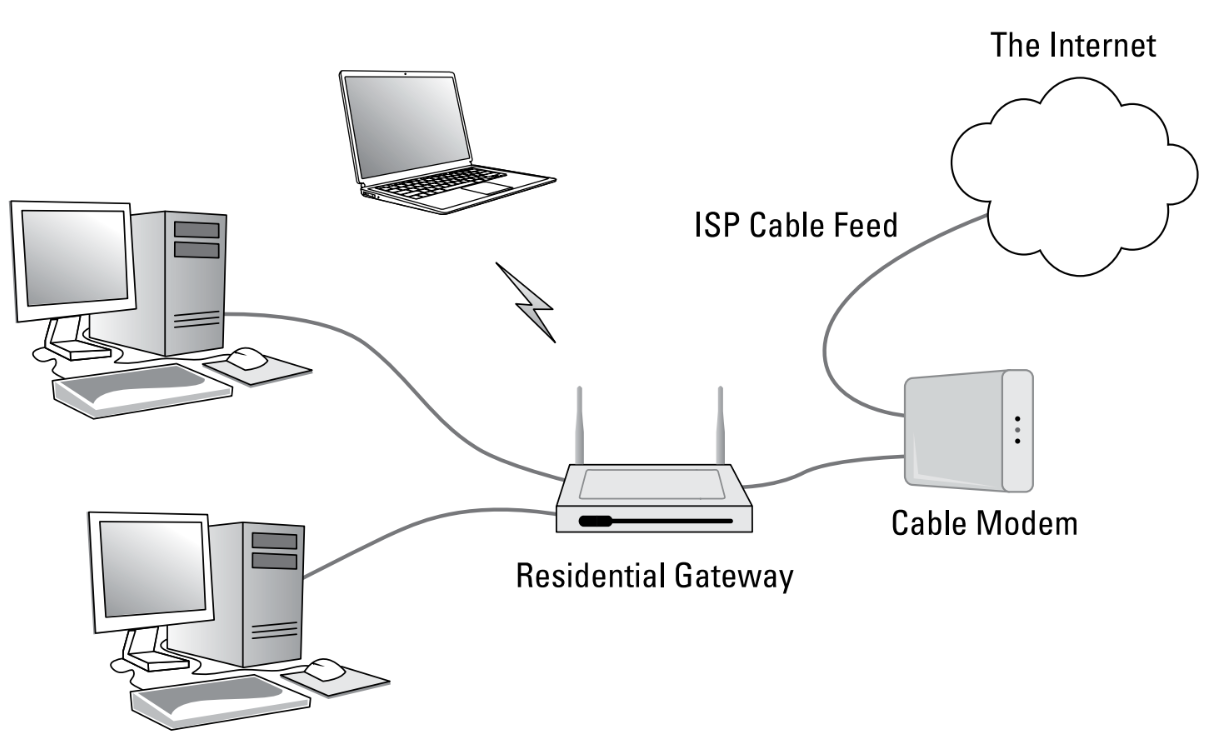
\includegraphics[width=0.8\textwidth]{fig/fig33}
	\caption{De vigtigste parametre for et datakommunikationskabel som lavpasfilter}
	\label{fig:low_pass_filter}
\end{figure}

\section{Fiberoptik}
Fiberoptiske kabler bruges normalt til at overføre digitale signaler over lange afstande med høj båndbredde. De har en kerne af rent optisk glas omgivet af en optisk kappe, der guider lysimpulser gennem kablet. Fiberoptik er mindre modtagelige for EMI og har en større informationsbærende kapacitet end kobberkabler.

\begin{figure}[h!]
	\centering
	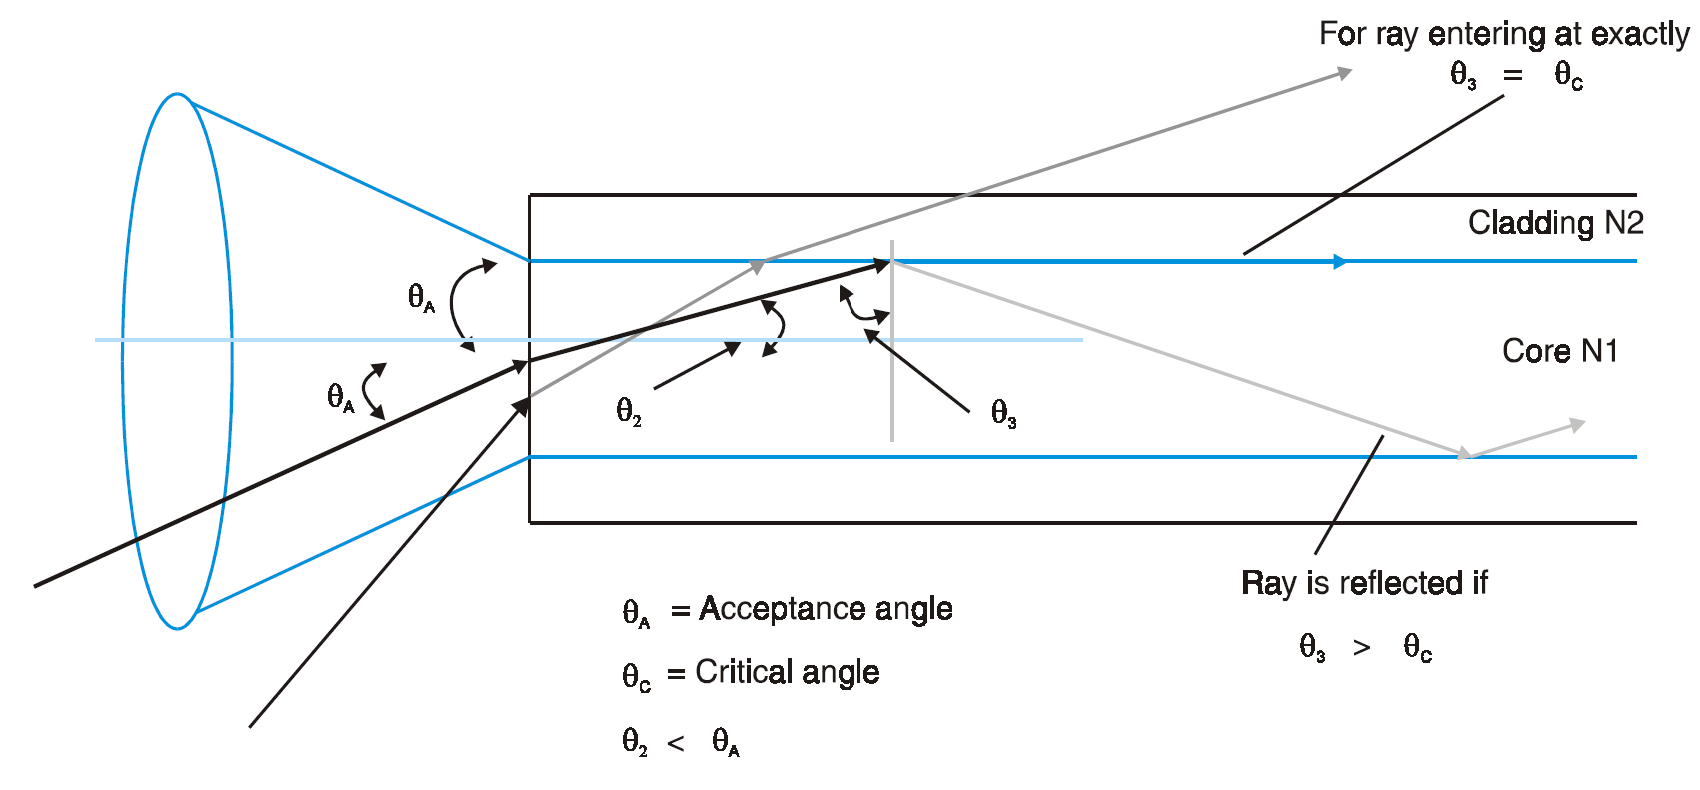
\includegraphics[width=0.8\textwidth]{fig/fig34}
	\caption{Opbygning af et fiberoptisk kabel}
	\label{fig:fiber_optic}
\end{figure}

\subsection{Driftsteori for fiberoptik}
Kommunikation over fiberoptiske kabler fungerer på princippet om, at lys bevæger sig gennem forskellige medier med forskellige hastigheder (på samme måde som radiobølger). Når lys bevæger sig fra et medium med en bestemt densitet til et andet med en anden densitet, ændrer lyset retning. Dette fænomen kaldes brydning.

\[
n = \frac{\text{Lysets hastighed i vakuum}}{\text{Lysets hastighed i mediet}}
\]

I et typisk fiberoptisk medium bevæger lyset sig ved cirka \(2 \times 10^8\) m/s. Brydningsindekset er derfor:

\[
n_1 = \frac{3 \times 10^8}{2 \times 10^8} = 1.5
\]

\begin{figure}[h!]
	\centering
	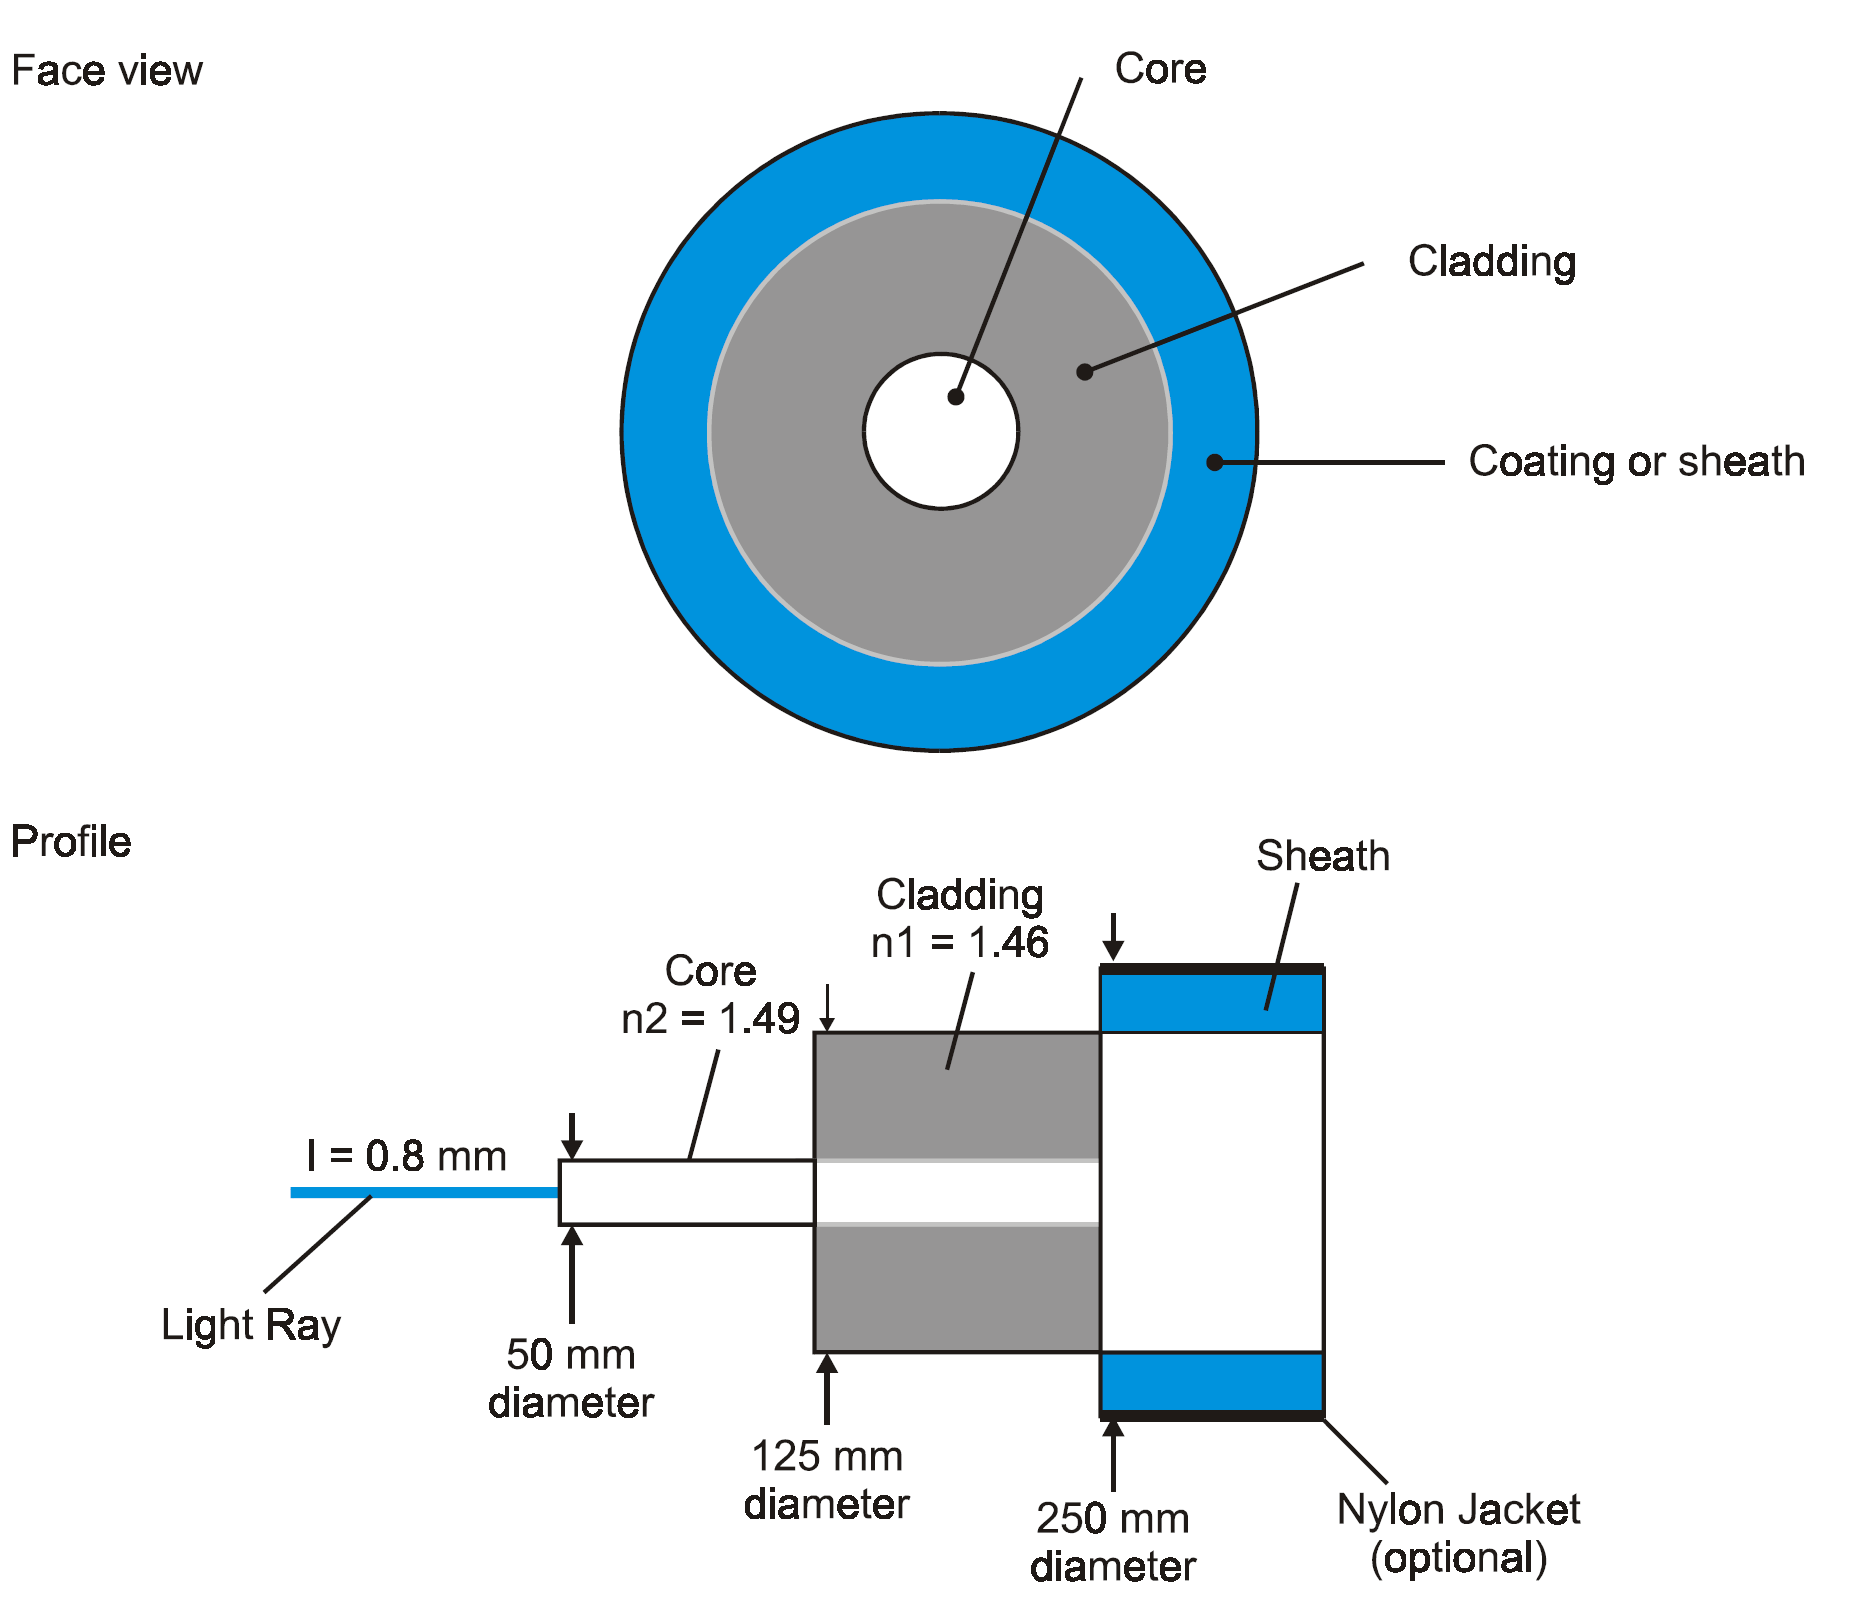
\includegraphics[width=0.7\textwidth]{fig/fig35}
	\caption{Optisk fiber principper}
	\label{fig:optical_fiber_principles}
\end{figure}

Den optiske fiber fungerer som en bølgeleder (eller lysleder) for lysimpulser genereret af en lyskilde. Lyskilden er typisk en laserdiode eller lysdiode (LED), der opererer ved bølgelængder på 0.85, 1.3 eller 1.55 mikrometer.

\begin{figure}[h!]
	\centering
	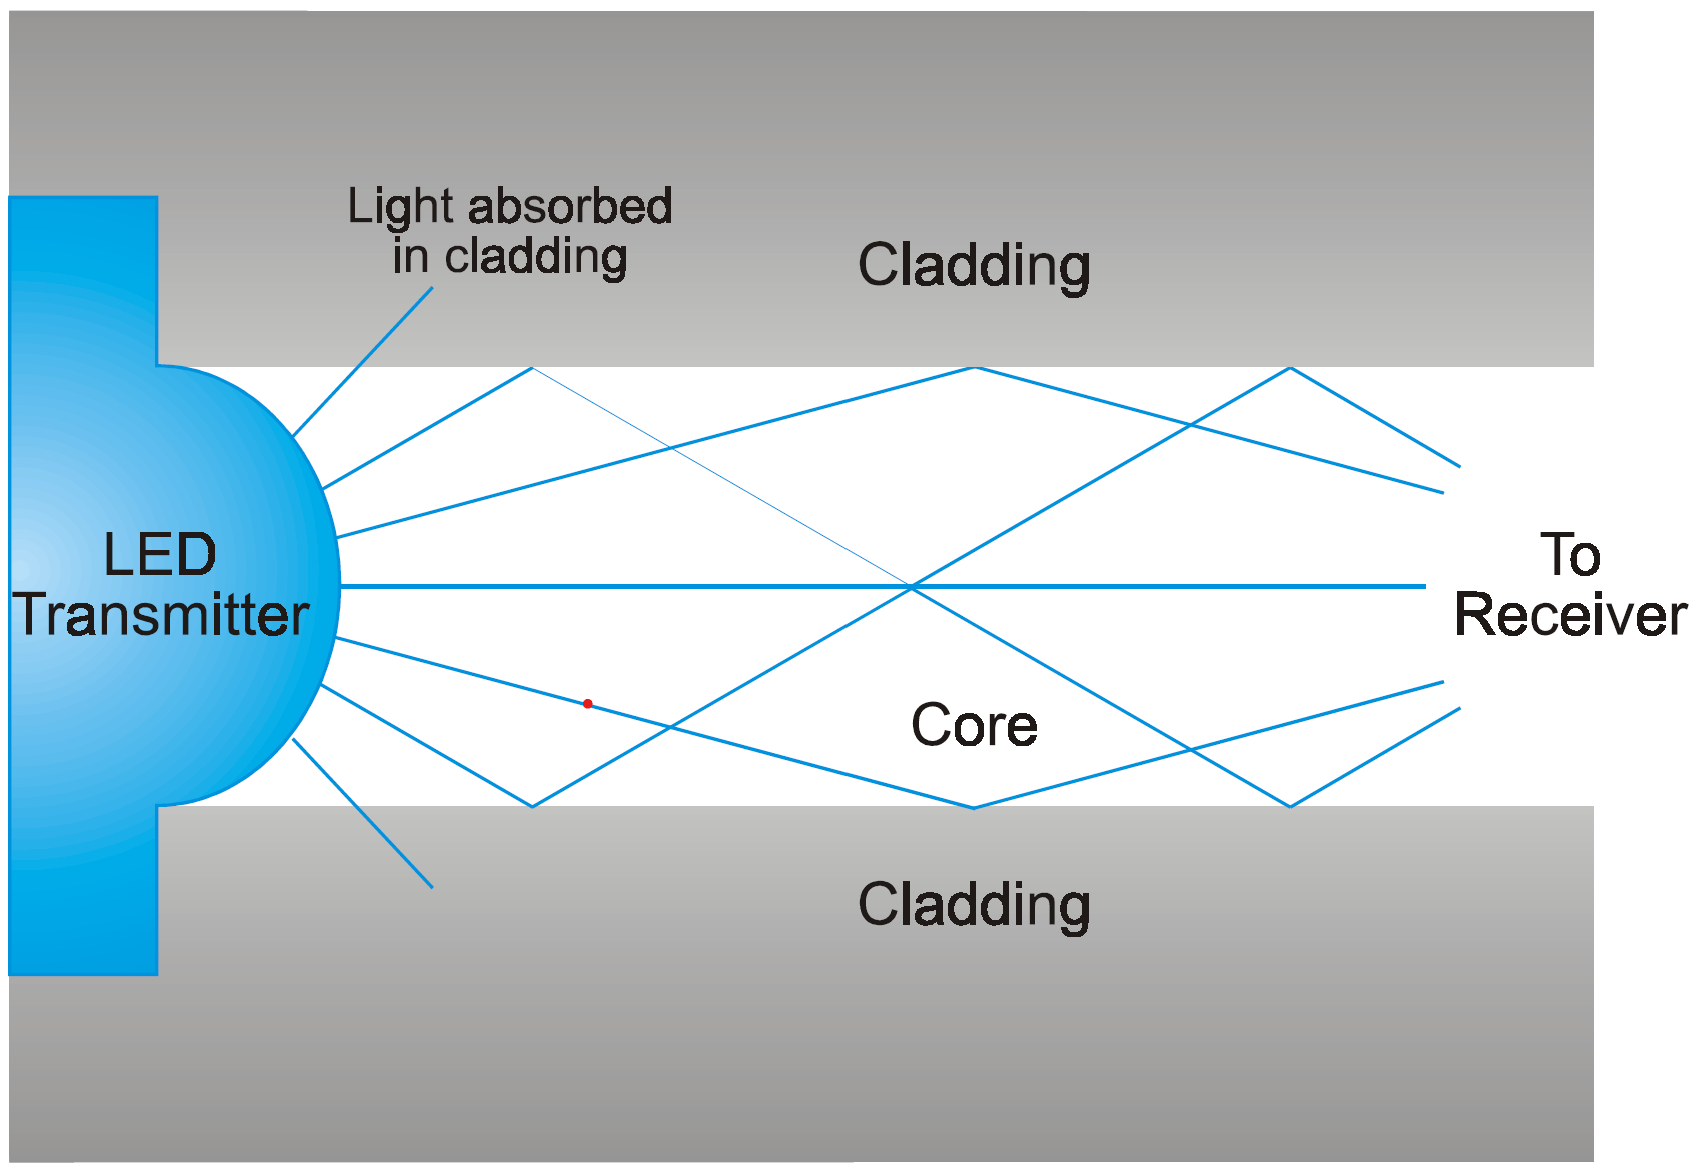
\includegraphics[width=0.6\textwidth]{fig/fig36}
	\caption{LED-lyskilde koblet til en multimode fiber (Step Index)}
	\label{fig:led_fiber}
\end{figure}

\subsection{Installation og vedligeholdelse}
Når Ethernet-kabler installeres, er det vigtigt at følge producentens specifikationer og industristandarder for at sikre korrekt ydeevne. Dette inkluderer korrekt bøjning af kabler, undgåelse af skarpe vinkler, og sikring af gode forbindelser i stik og patch paneler.
\newline
\newline
\noindent Vedligeholdelse af Ethernet-kabler omfatter regelmæssig inspektion for skader, sikring af korrekte forbindelser og opdatering af kablingsinfrastrukturen efter behov.

\subsection{Forbindelsestyper og Stik}
En korrekt installation af Ethernet-kabler inkluderer også valg af passende stik og forbindelsestyper. De mest almindelige typer af stik omfatter:
\begin{itemize}
	\item \textbf{RJ45-stik:} Det mest anvendte stik til Ethernet-forbindelser. RJ45-stik har otte ledere og bruges til at forbinde twisted pair kabler til netværksenheder som computere, routere og switches.
	\item \textbf{Andre stiktyper:} I specifikke applikationer kan andre stiktyper som RJ11, DB9, eller specialiserede industrielle stik være nødvendige.
\end{itemize}

\subsection{Ydeevne og Hastigheder}
Ydeevnen af Ethernet-kabler afhænger af kabeltypen og dens specifikationer:
\begin{itemize}
	\item \textbf{Hastighedskategorier:} Forskellige kategorier af twisted pair kabler (f.eks. Cat5e, Cat6, Cat6a, Cat7) tilbyder varierende niveauer af ydeevne i forhold til båndbredde og hastighed.
	\item \textbf{Maksimal Kabellængde:} For hver kategori af kabel er der en maksimal anbefalet kabellængde, som påvirker netværkets ydeevne. For eksempel er maksimal længde for Cat5e og Cat6 kabler 100 meter.
\end{itemize}

\subsection{Standarder og Protokoller}
Ethernet-netværk styres af en række standarder og protokoller, der sikrer kompatibilitet og ydeevne:
\begin{itemize}
	\item \textbf{IEEE 802.3:} Denne standard dækker de fleste aspekter af Ethernet-netværk og inkluderer specifikationer for forskellige hastigheder og medier.
	\item \textbf{Power over Ethernet (PoE):} PoE tillader samtidig overførsel af data og strøm via samme kabel, hvilket er nyttigt til enheder som IP-kameraer og trådløse adgangspunkter.
\end{itemize}

\subsection{Fejlfinding og Vedligeholdelse}
Regelmæssig vedligeholdelse og fejlfinding er afgørende for at opretholde et pålideligt Ethernet-netværk:
\begin{itemize}
	\item \textbf{Typiske Problemer og Løsninger:} Almindelige problemer inkluderer kabelbrud, dårlige forbindelser og interferens. Korrekt terminering og regelmæssig inspektion kan afhjælpe mange af disse problemer.
	\item \textbf{Testudstyr:} Kabeltestere og certificeringsværktøjer er vigtige for at verificere kabelintegritet og ydeevne. Disse værktøjer kan identificere problemer som krydsede par, åben kredsløb, og interferens.
\end{itemize}

\section{EMC (Elektromagnetisk Kompatibilitet)}
Elektromagnetisk kompatibilitet (EMC) er afgørende for at sikre, at elektroniske enheder og systemer kan fungere korrekt uden at forstyrre eller blive forstyrret af elektromagnetiske felter. I forbindelse med Ethernet-kabling er EMC vigtigt for at forhindre interferens, som kan påvirke signalintegriteten og netværkets ydeevne.
\begin{itemize}
	\item \textbf{Skærmning:} Shielded twisted pair (STP) kabler og korrekt jordforbindelse hjælper med at reducere EMI og forbedre EMC.
	\item \textbf{Kabelruting:} Undgå at placere Ethernet-kabler tæt på strømkabler eller andre kilder til elektromagnetisk støj.
	\item \textbf{Filter og Beskyttelse:} Brug af filtrerings- og beskyttelsesmekanismer kan hjælpe med at beskytte netværksenheder mod EMI.
\end{itemize}

\subsection{Sikkerhed og ydeevne}
Sikkerhed og ydeevne er afgørende faktorer ved installation af Ethernet-kabler i industrielle miljøer. Korrekt jordforbindelse og afskærmning skal implementeres for at beskytte mod EMI. Derudover skal kablerne være i stand til at opretholde datahastigheder og pålidelighed under alle driftsforhold.
\newline\newline\noindent 
Ved at følge disse retningslinjer kan en pålidelig og effektiv 
\newline\noindent Ethernet-netværksinfrastruktur etableres, som kan modstå de udfordringer, der findes i industrielle miljøer.

\chapter{Hardware Konfigurationer}
\section{Switch}
\section{Router}
